%%%%%%%%%%%%%%%%%%%%%%%%%%%%%%%%%%%%%%%%%
% Professional Formal Letter
% LaTeX Template
% Version 2.0 (12/2/17)
%
% This template originates from:
% http://www.LaTeXTemplates.com
%
% Authors:
% Brian Moses
% Vel (vel@LaTeXTemplates.com)
%
% License:
% CC BY-NC-SA 3.0 (http://creativecommons.org/licenses/by-nc-sa/3.0/)
%
%%%%%%%%%%%%%%%%%%%%%%%%%%%%%%%%%%%%%%%%%

%----------------------------------------------------------------------------------------
%	PACKAGES AND OTHER DOCUMENT CONFIGURATIONS
%----------------------------------------------------------------------------------------

\documentclass[12pt, a4paper]{letter} % Set the font size (10pt, 11pt and 12pt) and paper size (letterpaper, a4paper, etc)

%%%%%%%%%%%%%%%%%%%%%%%%%%%%%%%%%%%%%%%%%
% Professional Formal Letter
% Structure Specification File
% Version 1.0 (12/2/17)
%
% This file originates from:
% http://www.LaTeXTemplates.com
%
% Authors:
% Brian Moses
% Vel (vel@LaTeXTemplates.com)
%
% License:
% CC BY-NC-SA 3.0 (http://creativecommons.org/licenses/by-nc-sa/3.0/)
%
%%%%%%%%%%%%%%%%%%%%%%%%%%%%%%%%%%%%%%%%%

%----------------------------------------------------------------------------------------
%	PACKAGES AND OTHER DOCUMENT CONFIGURATIONS
%----------------------------------------------------------------------------------------

\usepackage{graphicx} % Required for including pictures

\usepackage[T1]{fontenc} % Output font encoding for international characters
\usepackage[utf8]{inputenc} % Required for inputting international characters
\usepackage{gfsdidot} % Use the GFS Didot font: http://www.tug.dk/FontCatalogue/gfsdidot/
\usepackage{microtype} % Improves typography
%\usepackage{setspace}
\usepackage{url}
\usepackage{rotating} 
% \usepackage{amsmath}
% \usepackage{amssymb}
\setlength\parskip{\bigskipamount} \setlength\parindent{0pt}
\usepackage{color}
% \usepackage{fontspec}


\pagestyle{empty} % Suppress headers and footers

\setlength\parindent{1cm} % Paragraph indentation

% Create a new command for the horizontal rule in the document which allows thickness specification
\makeatletter
\newcommand{\vhrulefill}[1]{\leavevmode\leaders\hrule\@height#1\hfill \kern\z@}
\makeatother

%----------------------------------------------------------------------------------------
%	DOCUMENT MARGINS
%----------------------------------------------------------------------------------------

\usepackage{geometry} % Required for adjusting page dimensions

\geometry{
	top=3cm, % Top margin
	bottom=3cm, % Bottom margin
	left=1.5cm, % Left margin
	right=1.5cm, % Right margin
	%showframe, % Uncomment to show how the type block is set on the page
}

%----------------------------------------------------------------------------------------
%	DEFINE CUSTOM COMMANDS
%----------------------------------------------------------------------------------------

\newcommand{\logo}[1]{\renewcommand{\logo}{#1}}

\newcommand{\Who}[1]{\renewcommand{\Who}{#1}}
\newcommand{\Title}[1]{\renewcommand{\Title}{#1}}

\newcommand{\headerlineone}[1]{\renewcommand{\headerlineone}{#1}}
\newcommand{\headerlinetwo}[1]{\renewcommand{\headerlinetwo}{#1}}

\newcommand{\authordetails}[1]{\renewcommand{\authordetails}{#1}}

%----------------------------------------------------------------------------------------
%	AUTHOR DETAILS STRUCTURE
%----------------------------------------------------------------------------------------

\newcommand{\authordetailsblock}{
	\hspace{\fill} % Move the author details to the far right
	\parbox[t]{0.48\textwidth}{ % Box holding the author details; width value specifies where it starts and ends, increase to move details left
		\footnotesize % Use a smaller font size for the details
		\Who\\ % Author name
		\textit{\authordetails} % The author details text, all italicised
	}
}

%----------------------------------------------------------------------------------------
%	HEADER STRUCTURE
%----------------------------------------------------------------------------------------

\address{
	\includegraphics[width=2.5in]{\logo} % Include the logo of author institution
	\hspace{0.82\textwidth} % Position of the institution logo, increase to move left, decrease to move right
	\vskip -0.05\textheight~\\ % Position of the large header text in relation to the institution logo, increase to move down, decrease to move up
	\Large\hspace{0.2\textwidth}\headerlineone\hfill ~\\[0.006\textheight] % First line of institution name, adjust hspace if your logo is wide
	\hspace{0.2\textwidth}\headerlinetwo\hfill \normalsize % Second line of institution name, adjust hspace if your logo is wide
% 	\makebox[0ex][r]{\textbf{\Who\Title}}\hspace{0.01\textwidth} % Print author name and title with a little whitespace to the right
	~\\[-0.01\textheight] % Reduce the whitespace above the horizontal rule
	\hspace{0.2\textwidth}\vhrulefill{1pt} \\ % Horizontal rule, adjust hspace if your logo is wide and \vhrulefill for the thickness of the rule
	\authordetailsblock % Include the letter author's details on the right side of the page under the horizontal rule
	\hspace{-0.25\textwidth} % Horizontal position of the author details block, increase to move left, decrease to move right
	\vspace{-0.1\textheight} % Move the date and letter content up for a more compact look
}

%----------------------------------------------------------------------------------------
%	COMPOSE THE ENTIRE HEADER
%----------------------------------------------------------------------------------------

\renewcommand{\opening}[1]{
	{\centering\fromaddress\vspace{0.05\textheight} \\ % Print the header and from address here, add whitespace to move date down
	\hspace*{\longindentation}\today\hspace*{\fill}\par} % Print today's date, remove \today to not display it
	{\raggedright \toname \\ \toaddress \par} % Print the to name and address
	\vspace{1cm} % White space after the to address
	\noindent #1 % Print the opening line
}

%----------------------------------------------------------------------------------------
%	SIGNATURE STRUCTURE
%----------------------------------------------------------------------------------------

\signature{\Who\Title} % The signature is a combination of the author's name and title

\renewcommand{\closing}[1]{
	\vspace{2.5mm} % Some whitespace after the letter content and before the signature
	\noindent % Stop paragraph indentation
	\hspace*{\longindentation} % Move the signature right to the value of \longindentation
	\parbox{\indentedwidth}{
		\raggedright
		#1 % Print the signature text
		\vskip 1.65cm % Whitespace between the closing text and author's name for a physical signature
		\fromsig \\% Prints the value of \signature{}, i.e. author name and title
		
\includegraphics[scale=0.25]{lmfcarvalho_sign.jpg}
	}
}
 % Include the file that specifies the document structure

\newcommand{\bibsection}[1]{}
\newcommand{\section}[1]{}
\newcommand{\newblock}{}

\newenvironment{thebibliography}[1]%
      {References\begin{description}}{\end{description}}
   \newcommand{\htmlbibitem}[2]{\label{#2}\item[{[#1]}]}
\usepackage[authoryear]{natbib}

\newenvironment{reply}{$\triangleright$\bf}{$\triangleleft$}
\renewenvironment{quote}
               {\list{}{\rightmargin\leftmargin}%
                \item\relax\normalfont}
               {\endlist}

\setlength\parskip{\bigskipamount} \setlength\parindent{0pt}

%\longindentation=0pt % Un-commenting this line will push the closing "Sincerely," and date to the left of the page

%----------------------------------------------------------------------------------------
%	YOUR INFORMATION
%----------------------------------------------------------------------------------------


\Who{Dr. Luiz Max de Carvalho} % Your name

\Title{, PhD} % Your title, leave blank for no title
\authordetails{
	School of Applied Mathematics\\ % Your department/institution
	Praia de Botafogo, 190\\ % Your address
	Rio de Janeiro, RJ, 22250-900\\ % Your city, zip code, country, etc
	Email: lmax.fgv@gmail.com \\ % Your email address
	Phone: +55 21 3799-2348 \\ % Your phone number
% 	URL: LaTeXTemplates.com % Your URL
}

%----------------------------------------------------------------------------------------
%	HEADER CONTENTS
%----------------------------------------------------------------------------------------
\logo{emap.png}
% \logo{Marca_FGV_EMAp_colorida.png}

\headerlinetwo{Getúlio Vargas Foundation (FGV)} % Top header line, leave blank if you only want the bottom line

% \headerlinetwo{School of Applied Mathematics (EMAp)} % Bottom header line

%----------------------------------------------------------------------------------------

\begin{document}

% Template for PLoS
% Version 1.0 January 2009
%
% To compile to pdf, run:
% latex plos.template
% bibtex plos.template
% latex plos.template
% latex plos.template
% dvipdf plos.template

\documentclass[10pt]{article}
\usepackage{amsmath}
\usepackage{amssymb}
\usepackage{graphicx}
\usepackage{color} % for revision purposes only, may be not present in the final file
% cite package, to clean up citations in the main text. Do not remove.
\usepackage{cite}
\usepackage{color}
\usepackage{indentfirst} %% LM: in order to indent the first paragraph of each section
\usepackage{url} %% LM: in order to include nice urls
\usepackage{booktabs} %% LM: nice tables...
\usepackage{subfigure} % LM: panels
% Use doublespacing - comment out for single spacing
%\usepackage{setspace}
%\doublespacing

\topmargin 0.0cm
\oddsidemargin 0.5cm
\evensidemargin 0.5cm
\textwidth 16cm
\textheight 21cm

\usepackage[labelfont=bf,labelsep=period,justification=raggedright]{caption}

\bibliographystyle{plos2009}% 


\makeatletter
\renewcommand{\@biblabel}[1]{\quad#1.}
\makeatother


% Leave date blank
\date{}

\pagestyle{myheadings}
%% ** EDIT HERE **


%% ** EDIT HERE **
%% PLEASE INCLUDE ALL MACROS BELOW

%% END MACROS SECTION

\begin{document}

% Title must be 150 characters or less
\begin{flushleft}
{\Large
\textbf{Spatiotemporal Dynamics of Foot-and-mouth Disease Virus in South America}
}
% Insert Author names, affiliations and corresponding author email.
\\
Luiz Max Fagundes de Carvalho$^{1\ast}$,
Guy Baele$^{2}$,
Nuno Rodrigues Faria$^{2,3}$,
Andres M. Perez$^{4}$,
Philippe Lemey$^{2}$,
Waldemir de Castro Silveira$^{1}$
\\
\bf{1} Pan American Center for Foot-and-Mouth Disease (PAHO/WHO), Duque de Caxias, Rio de Janeiro, Brazil
\\
\bf{2} Department of Microbiology and Immunology, Rega Institute, KU Leuven, Belgium
\\
\bf{3} Department of Zoology, University of Oxford, Oxford OX1 3PS, UK
\\
\bf{4} Center for Animal Disease Modeling and Surveillance, University of California at Davis, Davis, United States of America
\\
$\ast$ E-mail: lcarvalho@paho.org
\end{flushleft}

% Please keep the abstract between 250 and 300 words
\section*{Abstract}

JUST IN THE END :)\\

Key-words: Phylogeography, foot-and-mouth disease virus, South America, animal trade, BEAST.

\section*{Introduction}

Foot-and-mouth disease virus (FMDV) is a rapidly evolving picornavirus, causative agent of the most important disease of domestic and wild cloven-hoofed animals, foot-and mouth disease (FMD) \cite{review}.
FMD is endemic in several regions of South America, and in recent years, the circulation of three of the seven FMDV serotypes, namely serotypes C, A and O, has been reported in the continent, the later two being the most prevalent.
%NRF perhaps you can drop here some references about serotype distribution in SAmerica
Serotypes A and O show different  geographic distribution, with O being more prevalent in endemic Andean areas \cite{andean} and A being responsible for sporadic outbreaks in the Southern cone \cite{Perez2001,Malirat2012}.
%NRF emergences=outbreaks?
FMDV has probably been introduced in South America in the late years of the 19th century, probably brought by European colonization \cite{tully}. 
By the 1970's, FMD was widespread in South America, with occurrence of multiple subtypes in large-scale epidemics \cite{Saraiva2003}.
As a consequence of the improving knowledge about disease ecosystems accumulated by the national programmes, the Hemispheric Plan for the Eradication of FMD (PHEFA) was launched in 1987.
PHEFA was elaborated and signed by South American countries as a continent-wide programme to strenghten national infra-structures, control animal trade and improve diagnostic and epidemiological investigation capabilities \cite{review_eradication}.
Its main objective is to create and maintain FMD-free areas, thus improving the availability of meat, milk and other economically important livestock products \cite{Saraiva2003,Saraiva2004,review_eradication,combining}. Considerable success has been achieved over the past years, with substantial reduction of FMD incidence in the late 1990's.
Nevertheless, episodic outbreaks in 2001, 2005 and 2011 in previously free areas represented a serious setback to PHEFA, which was devised to fulfill its goals by 2010 \cite{Saraiva2003,Saraiva2004}.

The generally accepted solution to the problem of FMD eradication involves the promotion of transnational massive vaccination programmes \cite{vaccinationSA}
with the development of better veterinary surveillance systems. Phylogenetic analyses have already proved useful in the latter, particularly by recovering in real-time the transmission pathways from genetic data \cite{cottam2008} and providing insight into the processes that drive re-emergence \cite{combining}.
In the South American ecotone, the molecular evolution of FMDV has been subject of several studies along the years \cite{Perez2001,Malirat2007,andean,Malirat2011,Maradei2013}.
These studies have played an important role in understanding the (re-)emergence pattern of FMDV, allowing for inference on the origin and evolutionary history of emerging viral strains \cite{topotypes,Perez2001}. Together with vaccine matching and MAb profiling studies \cite{Maradei2011}, phylogenetic analyses are a powerful 
tool to evaluate control programmes and guide vaccine formulation \cite{Maradei2011,Maradei2013}.

The increased availability of geo-referenced time-stamped genetic data has fostered the development of new methods that integrate epidemiological and environmental data in order to reconstruct pathogen population dynamics and test evolutionary hypotheses \cite{MEP,grenfell}. 
However, and as pointed out by Di Nardo, Knowles \&  Paton (2011) \cite{combining}, this joint evaluation of information from different sources is usually done outside of a unified quantitative framework, and in a qualitative fashion. In this context, Bayesian phylogeography offers a statistical framework to jointly combine multiple sources of information in order to understand the spatio-temporal dynamics of FMDV and perform evolutionary hypothesis testing. Such framework recently proven useful when investigating the patterns of FMDV spread and trace the spatial origins of FMD epidemics \cite{Carvalho2012,bulgaria,phymal,hall2013}.

In this study we apply state-of-art Bayesian phylogeographic methods
to investigate the evolutionary dynamics of serotypes A and O in South America, both in a spatial and temporal perspective. The probabilistic framework used here allows for the incorporation of multiple sources of information to test hypothesis about viral dispersal, while naturally accommodating uncertainty \cite{roots,towards}.
We use BEAST \cite{beast2012} to build time-structured phylogenies and a recent demographic growth model \cite{skyride} to reconstruct past population dynamics, to which we overlay with vaccination and serotype-specific notification data.
Moreover, we use data on livestock trade and geographical distances as predictors for viral spatial diffusion and use recently developed methods to accurately calculate marginal likelihoods for each predictor.
Finally, we offer an appreciation of the statistical hurdles that may be caused by biased geographic sampling, and propose ways to ameliorate their effects.
%TODO: decide whether or not this statement holds in the end
\section*{Results}

\subsection*{South American FMDV serotypes A and O exhibit rate variation among lineages and evolve measurably}

In this study, we analyzed all publicly available VP1 (1D) sequences for serotypes A and O in South America (131 and 167 sequences, respectively) using a Bayesian phylogeographic approach. Our data sets spanned over a large period (1955-2010 for serotype A and 1994-2010 for serotype O)  and covered nearly all South American countries affected by FMD.

First, jModelTest selection analysis yielded the general time reversible (GTR) model with a discretized gamma distributed across-site rate variation and a proportion of invariant sites (GTR+I+$\Gamma_{4}$) model as the best fit nucleotide substitution model for both FMDV data sets.
Next, we performed a stringent model selection analysis to chose the best-fit demographic growth model and molecular clock model.
Our results indicate that the constant population assumption is decisevely rejected (A: BF=$11$; O: BF= $21$) in favour of a model that allows fluctuations in demographic growth over time. 

After, we found that both serotypes A and O rapid evolution better fits a relaxed than strict molecular clock model.
Particularly, the exponential relaxed molecular clock provided a better fit for serotype O data (BF=$21$) while the lognormal relaxed molecular clock model provided a better fit to serotype A (BF=$11$) (see Table S1 for details).
% TODO: check this numbering
The coefficient of variation for the relaxed molecular clock models was estimated at $0.32$ (95\% BCI: $ 0.21$--$0.43$) and $0.99$ (95\% BCI: $0.90$--$1.08$) respectively for serotype A and O, indicating substantial rate heterogeneity among lineages in the phylogeny. 

We also performed a `temporal signal' test to evaluate the degree to which genetic divergence accumulates over time (described in \cite{Faria2012}).
This confirmed significant temporal signal for both serotypes (A: BF=$310$; O: BF=$348$), showing that both FMDV data sets analyzed here are measurably evolving populations.
Overall, these results show that sufficient temporal information is embedded in sequence data of both serotypes under investigation, which is central for the estimation of times of divergence and to reconstruct the population dynamics in natural time units \cite{MEP}.

\subsection*{Dating the divergence of FMDV in South America}

To build time-structured phylogenies for each FMDV serotype, we performed Bayesian MCMC analysis using BEAST, under the corresponding best-fit combination of nucleotide subsitution, demographic and molecular clock models.
The maximum clade credibility (MCC) tree estimated for serotype A (Figure~\ref{fig:trees}A) places the origin of the circulating strains in or around the early years of the 1920's decade.

Figure~\ref{fig:trees}A shows that sequences from the same country tend to cluster in small clades although the Bayesian phylogenies for both serotypes also shows considerable interspersing of lineages indicating trans-border FMDV migration.
For example, for serotype A sequences from Argentina are grouped in 2 clades that either comprised only Argentinian isolates or include sequences from Brazil and Uruguay (Figure~\ref{fig:trees}A).
Interestingly, the great majority of the isolates from Venezuela and Colombia fall together within 2 distinct clades. 

Figure~\ref{fig:trees}B presents the estimated MCC tree for serotype O.
The same interspersing pattern can be noticed, with Ecuador and Colombia showing several interleaved clades.
The TMRCA for serotype O was estimated in around 20 years, showing a more recent origin.
Here, a smaller clade of Colombian isolates are found interspersed within from Venezuelan isolates. In addition, isolates from Ecuador are found interspersed with isolates from Colombia, suggesting that the intra-country dynamics of FMDV between these two countries is intrinsically linked.
Overall, the Bayesian phylogenies suggest that most FMDV flow within South America occured between neighboring countries. 

Using the best fitting demographic and molecular clock model combination for each serotype, the evolutionary rate for serotype A was estimated around $4 \times 10^{-3}$ substitutions/site/year. In addition, the estimated evoltutionary rate for serotype O was aproximately 2.5 times faster than serotype A, i.e. at $1 \times 10^{-2}$, consistent with previous studies \cite{tully,Carvalho2012}. 

\begin{center}
 [Figure~\ref{fig:trees} about here]
\end{center}

\subsection*{Spatial Dynamics of FMDV in South America}

To assess the spatial pattern of FMDV spread within South America, we performed Bayesian phylogeographic analysis, also using the models available in BEAST \cite{roots}.
We began by evaluating the spatial signal contained in our sequences using Bayesian tip-association tests \cite{bats} to determine the amount of spatial signal in our reconstructed phylogenies.
To gain insight into the amount of association for each location, we computed the maximum clade (MC) statistic.
The results can be found in Table S2 and show significant location-tip association for both serotypes.
%TODO: check this numbering in the end.
MC statistics were different for each country in each dataset, showing different geographic structures for each serotype.
As an overall result, our datasets presented high degree of spatial signal, what justifies more complex phylogeographic analyses to study the transmission network of FMDV in the continent.

Fist, we employ an asymmetric continuous-time Markov chain (CTMC) phylogeographic model \cite{roots} to gain insight into the spatio-temporal process of FMDV spread. Coupled to this analysis we set up a Bayesian Stochastic Search Variable Selection (BSVSS) procedure to search for the most parsimonious set of migration routes (network edges) needed to explain the diffusion process (see Methods).
BSSVS also naturally allows for the computation of Bayes factors, which are in turn used to assess the importance/significance of each migration path.
The results are presented in Figure~\ref{fig:migration} and show that Brazil and Colombia were the most probable origins for serotypes A and O respectively.

For serotype O the highest rates were estimated for transitions between Argentina and Peru, Argentina and Venezuela, Uruguay and Ecuador and Uruguay and Argentina. When we analyzed the obtained Bayes factors, the best supported (BF$>9$) routes were between Peru and Brazil, Bolivia and Colombia, Argentina and Venezuela, Uruguay and Argentina and Argentina and Peru. The route between Uruguay and Peru showed smaller but strong support (BF$>4$).

The highest rates for serotype A were obtained for transitions between Brazil and Uruguay, Ecuador and Venezuela and Bolivia and Venezuela. When we looked at BF support we found the transitions between Argentina and Venezuela, Uruguay and Argentina, Argentina and Bolivia, Brazil and Argentina and Bolivia and Venezuela to have the highest Bayes factors (BF$>8$).

We can notice that for serotype A mainly long-range migration routes were inferred for the period before 1945.
This results may be due to sparsity of information before 1970, which precludes accurate inference about periods further back in time. 
Also, there is a major expansion in spatial spread from 1945 to 1965, characterized by Brazil as a source of virus for the rest of the continent.
In the period 1965-1980, we notice slower spread, mainly through short range routes.
The 1980-2008 window is characterized by FMDV serotype A flow into Peru and Paraguay and the increase of intra-country diversity (depicted by the radius of the displayed circles in Figure~\ref{fig:migration}).   

On the other hand, for serotype O expansion seems to have occured by the middle of the 1990 decade.
Up to 1995, Colombia and Brazil seem to have acted as primary and secondary viral sources, respectively.
From 1995 to 2000, whilst Colombia acted as main source for the northern/andean regions of the continent, spread in the Southern Cone seems to originate in Brazil.
The period 2000-2010 is characterized by a decrease in viral flow (almost no new edges added to the network) and the main feature is the increase in viral diversity within countries, specially Ecuador, Colombia and Brazil.

\begin{center}
 [Figure~\ref{fig:migration} about here]
\end{center}

To further explore the spatial behavior of FMDV we employ the so-called ``Markov jump'' counts \cite{Minin2008} of the expected number of location state transitions along the  branches of the phylogeny, which  provide a quantitative measure of gene flow between countries, representing successful viral introductions from one region to another. For this analysis we also calculated BF's using BSSVS.
The results are presented in Figure~\ref{fig:mj&BFs} and show that supported migration routes differ for each serotype, with some overlapping in the routes connecting Venezuela, Colombia and Ecuador.
For serotype A, highest (BF $>800$) support was observed for viral flow between Venezuela and Colombia and between Argentina and Uruguay.
Transitions between Brazil and Bolivia and Peru and Ecuador also received good statistical support (BF $>10$).
For serotype O, overall Bayes factors were lower in magnitude, but supported similar routes.
Highest support was found for transition between Ecuador and Peru and Colombia and Ecuador (BF $>100$). Signicant support was also observed for viral exchange between Venezuela and Colombia (BF $>20$). 

% Lots of short range routes are supported for both serotypes
% How to reconcile these results with the border vs non-border results below?

To further study this pattern, we compared the counts between countries that share borders and those which do not.
The results show that for serotype A the median transition count between neighbor countries was $0.02$ (95 \% BCI: $0.00$ -- $4.29$), while ``non-border'' transitions had median $0.05$ (95 \% BCI: $0.00$ --  $3.39$).
For serotype O, similar results were observed, with $0.04$ ($0.00$ -- $1.99$) and $0.09$ ($0.00$ -- $1.25$) being observed for neighboring and non-neighboring countries, respectively.
Since the difference in medians is substantial but quantiles widely overlap, we set up a Monte Carlo resampling experiment to calculate the probability that a randomly chosen ``border'' ($B$) transition is larger than a randomly chosen ``non-border'' ($NB$) one. For each data vector we obtained $10,000$ random draws and counted the number of times the above described event happened. From this experiment we found $Pr(B>NB)$  to be $0.41$ for serotype A and $0.36$ for serotype O.

\begin{center}
 [Figure~\ref{fig:mj&BFs} about here]
\end{center}

One may ask if both serotypes present different spatial spread patterns.
To assess this we used PS/SS to calculate marginal likelhihoods for two different models, henceforth  called ``shared'' and ``separate''.
In the ``shared'' model we used trait (location) and sequence data  from both serotypes to make inference about one CTMC rate matrix, whilst in the ``separate'' model we allow both serotypes to have each one CTMC rate matrix, while using the combined data from both serotypes.
Both models allow serotypes to have different spatial diffusion rates.

We plotted the rates estimated from independent runs for both serotypes and they do not seem to correlate (Fig. S3). % TODO: check this numbering in the end
Moreover, from the separate and shared rate matrix analysis we found that rates inferred for serotype A are more strongly correlated with the rates estimated under a shared rate matrix, with Pearson's linear correlation coefficients $r_A=0.55$ and $r_O=0.18$, respectively.
For this analysis, the correlation between serotype A and O rate matrix estimates was $0.07$.
In contrast to these results, the rate indicators in BSSVS for both serotypes were in better accordance ($r=0.54$).
Again, we compared estimates using shared and separate models for the CMTC rate matrix, and found that indicators for serotype A had higher concordance to those in the shared model ($r_A=0.86$ and $r_O=0.77$).
Bayes factors assessment of the statistical support for the two hypotheses (shared or separate rate matrices), indicated that a shared model should be preferred to a model with separate rate matrices for each serotype (BF$>10$, see Table~\ref{tab:sharedsep}).

% TODO: are the shared runs more statistically efficient? 
\begin{center}
 [Table~\ref{tab:sharedsep} about here]
\end{center}

\subsection*{Identifying potential predictors of FMDV spread in South America}

We used data from the detailed trade matrix available from the Food and Agriculture Organization (FAO) to elicit CMTC rate matrix priors (predictors).
By accurately calculating the marginal likelihood of each predictor we can gain insight into the importance of each predictor on viral spread \cite{Carvalho2012,Nelson2011}.
We used data on geographic distances and on trade of live cattle, pigs and sheep.
For each predictor, we also performed a MCMC run using sampling-corrected base frequencies for each country.
All predictors were compared to a spatially uniform vague prior using Bayes factors.

Interestingly, the results of this analyses (Table~\ref{tab:preds}) show different best fitting predictors for each serotype.
While for serotype A the best predictor was the trade of live sheep between countries (BF$=20$), the exchange of cattle was the best predictor for serotype O spread (BF$=6$).
Undecisive support (BF$=2$) was also observed for the trade of live pigs.
Also, while for serotype A we found moderate statistical support for geographic distances as predictors of viral spread (BF$=4$), this predictor was not identified for serotype O.
%TODO: decide what to do with the freq runs

%NRF Do have any results for the analyses combining the rate matrices of O and A? What was the best fitting predictor in this case?
% LM Nope we don't, unfortunately :(
\begin{center}
 [Table~\ref{tab:preds} about here]
\end{center}

For each predictor we also assessed the state distribution at root, i.e., the probability of each country being the origin of the circulating strains.
In Table~\ref{tab:roots} we show that for serotype A there was discordance between predictors about which country was the most probable source of FMDV in the continent.
Peru was the most probable location of origin for most of the predictors, but notably not for the best fitting predictor (sheep trade), for which Brazil was estimated as the origin with high probability ($0.90$).
For the pigs trade predictors, Colombia was found to be the spatial origin.

For serotype O, showed much more concordance, and Colombia was pointed out as the spatial viral origin for all predictors with high probability (Table~\ref{tab:roots}).

\begin{center}
 [Table~\ref{tab:roots} about here]
\end{center}
\subsection*{Sampling bias assessment in the phylogeographic analysis}
Since our data sets presented highly preferential sampling, we conducted a detailed sensitivity analysis to assess the effect of performing inference under highly unbalanced designs.
% TODO: include the BF test using rep-informed priors
First, we draw five subsamples for each serotype in which overrepresented were downsampled and performed BSSVS for each subsample.
From BSSVS we calculated Bayes factors and observed good agreement between samples in terms of supported routes (see Figures S4 and S5). % TODO: check this numbering in the end    
To further study this, we also computed the $L1$ and $L2$ matrix distance norms for across the estimated rate matrices for each subsample, and no aberrant samples were detected.

Another aspect of interest is the amount of information extracted from each sample, which we measure by calculating Kullback-Leibler divergence between prior and posterior distribution of traits at root \cite{roots}.
Tables S3 and S4 show that for all subsamples in both serotypes there was substantial information extraction, with highly concentrated posterior distributions at root.
Inference about location of origin was consistent across samples, with Brazil and Colombia being the countries of origin for serotypes A and O respectively.
Also, we observed stronger support for Colombia as root for serotype O when compared to Brazil as root for serotype A.
While serotype O presented average $Pr(\text{root=Colombia})=0.95$, $Pr(\text{root=Brazil})$ for serotype A was $0.83$.
% TODO: check this numbering in the end
\subsection*{Demographic reconstruction of FMDV dynamics}

The results from the Skyride coalescent reconstruction show strikingly different dynamical behaviors for the two serotypes, with serotype O exhibiting considerable more oscillation over time, and a diversity peak occurring in late years of the 1990 decade.
Serotype A exhibits a more stable behavior over most of the 20th century, with most variation occurring within the temporal sampling interval, mainly in the last years of the 2000 decade.
To better understand the relationship between vaccination and viral diversity, we overlaid vaccination data to our skyride plots presented in Figure~\ref{fig:skyride}.
These data were expressed as doses per head, which we consider to be a more accurate measure of vaccination coverage, since it corrects for population size increase/decrease over time (see Figure S1 for livestock population and trade time series). %TODO: check this numbering in the end
Also, serotype-specific disease notification data was collected and plotted as an overlaid time series to the reconstruction. 

To assess the robustness of our reconstructions we performed skyride reconstructions using only recent (sampling date $>2000$) sequences (see Text S2, Figure S6).
%TODO: Check this numbering in the end
We also performed reconstructions in datasets without the over-represented locations (data not shown). All these analyses gave roughly similar results to those presented in Figure~\ref{fig:skyride}. The only exception was the reconstruction for serotype A without Argentinian sequences, for which it is not possible to see the marked drop near 2001 that is clear in Figure~\ref{fig:skyride}. 

\begin{center}
 [Figure~\ref{fig:skyride} about here]
\end{center}

\section*{Discussion}
%%%%
% PHYLOGENETIC ANALYSIS
%%%%
Bayesian phylogenetics provides a framework for rigorously testing evolutionary hypotheses without conditioning on a single tree topology. Hence, this approach naturally accommodates phylogenetic uncertainty and, combined with accurate methods for marginal likelihood calculation, perform Bayesian model selection \cite{Baele2012,Baele2013a,Baele2013b}.

%  Interestingly, best fit branch substitution models (molecular clock) were different for both serotypes (Table S1) suggesting different evolutionary dynamics
Thus, while for serotype A a more restrictive exponential molecular clock and a slower mutation rate were found, for serotype O our results point out a more diffuse distribution of branch-specific substitutions (lognormal) and a faster evolutionary rate.
The differences in evolutionary rates, when taken together with the results from molecular clock model selection, suggest that, although the two serotypes share the same host and infection routes, they present rather different evolutionary dynamics. 

%%%%%
%SPATIAL DYNAMICS
%%%%
% As discussed by Cottam et al (2007) \cite{cottam2007}, phylogenetic methods can be used to unravel undetected transmission.
% We focus on a comparative approach, using information obtained from both serotypes to gain insight into the general process of FMDV spread in South America.
%This continent wide-sampling allowed us to reconstruct the temporal and spatial dynamics of FMDV in the continent for both serotypes in greater detail than previous studies
% Ecuador is a BF star, key to the spread, endemic country
% For serotype O, Colombia is north, Brazil is south.
% These countries share borders and have similar enviromental conditions 
% TODO: do they?
% serotype A expansion took place mostly in the early years of the 20th century and expansion for serotype O occured in the beggining of the 1990 decade.
% Although both serotypes have different tempo, several spread routes were found in both migration networks. As an important difference...
% the relationship between MJ borders inference and source-sink dynamics
% Discrepancy between highest rates and highest BFs
% Border vs non-border suggests long-range stuff may be important as well.
% REMEMBER TO DISCUSS SHARED VERSUS SEPARATE ANALYSES. shared vs separate reveal that spatial spread is quite the same
% Our results suggest that FMDV serotypes have same dispersal determinant
% when we analyzed INDICATORs  much higher concordance
% Notably, Venezuela, Colombia and Ecuador form a densely connected sub-network for both serotypes.
%%%%%
% PREDICTORS
%%%%%
The ability to incorporate multiple sources of information like temporal and spatial data is becoming increasingly important in molecular epidemiology studies that aim to understand the driving forces of pathogen evolution and spread \cite{towards,combining,MEP,roots}. 
Using animal trade data as predictors can be a valuable tool to understand the role of livestock commerce in the spread of animal and zoonotic diseases \cite{Nelson2011}.
We found significant well supported migration paths between Venezuela, Colombia and Ecuador for both serotypes and this may indicate...??
% LM differet predictors = different roots <- What to do?
% These results help to shed light into the main determinants of viral flow in the continent.
% selection of clock and tree prior by PS/SS is cumbersome, but provides more accurate results. This calls for better methods, specially tailored for phylogeography 
% TODO: LM What does Guy think about this?
%%%%%
% SAMPLING BIAS
%%%%%
% Informing the rates with livestock trade contributes to ameliorate the bias introduced by unbalanced sampling in the sense that it allows for an external source of information to be incorporated \cite{Faria2012}.
% TODO: include polar bear citation and talk about sensitivity analysis
%%%%%
% COALESCENT 
%%%%%
It can be noticed from both serotypes that over time, with the increase of vaccination coverage, viral effective population size ($Ne$) decreases dramatically.
This drop is also present in FMD notifications, what may suggest the role of epidemics in viral diversity.
These results draw an interesting picture: over the years vaccination seems to be disrupting viral diversity, supposedly by precluding spread over large spatial extents, inducing a state of focalized transmission [NEED A REF HERE].

In order to strenghten epidemiological inference, it may be interesting to compare the results obtained for both serotypes.
Serotype O presents more estable temporal behavior, whereas serotype A is more fluctuating.
Previous studies have shown that occurences caused by serotype A present longer cycles and wider epidemics, while serotype O is more prevalent with shorter disease cycles \cite{colombiatime}.
These epidemiological features are reflected at the temporal variation observed for viral $Ne$ in both serotypes, a result obtained for other viruses as well \cite{Bennett2010,Pybus2003}. 
Since our results reinforce the notion that these two serotypes present different evolutionary dynamics, the overall decrease in viral diversity for both serotypes points towards a progressive success of the eradication programme in slowly reducing transmission and controlling epidemics.
% in the future skyride reconstructions can be coupled to mathematical models to help explain the pattern of emergence of FMD
\section*{Conclusions}
% can be used to infer host jumps \cite{hall2013}
%better methods yield more complete analyses
%overall decrease in viral diversity
%spatial routes by proximity
%sampling bias may be an important factor to consider
% subsampling improved root estimation
\section*{Methods}

\subsection*{Genetic and epidemiological data}

To study the spatio-temporal spread dynamics of FMDV within South America we compiled the largest database of 1D (VP1) gene sequences to date for serotypes A and O.
We retrieved all 1D (VP1) nucleotide sequences available from the National Center for Biotechnology Information (NCBI, \url{ http://www.ncbi.nlm.nih.gov/}) for which there was information on country and year of isolation.
This resulted in 131 sequences (eight countries) for serotype A and 167 sequences (nine countries) for serotype O, covering time spans of 55 (1955-2008) and 16 (1994-2010) years, respectively (see Text S1 for details).
Each dataset was aligned using the MUSCLE \cite{muscle} algorithm implemented in the MEGA5 \cite{MEGA} package.

Data on animal trade were obtained from the FAO database (\url{http://faostat.fao.org/}).
We retrieved data on the detailed trade matrix for cattle, pigs and sheep (live animals) covering the period from 1986 to 2009, for each of the nine countries.
Serotype-specific outbreak notifications were obtained from FMD Bioportal (\url{http://fmdbioportal.ucdavis.edu:8080/}).

\subsection*{Phylogenetic Analysis}

First, we checked both data sets for recombination using the tools (SBP and GARD \cite{sbpgard}) available from the Datamonkey facility (\url{http://www.datamonkey.org/}), and no recombination was found.
We then used hierarchical likelihood model selection, as implemented in the package jModeltest 0.1.1 \cite{jmodel}, to select the best nucleotide substitution model for each data set.

We performed Bayesian model selection to assess the performance of different demographic and molecular clock models.
To this end, we used state-of-the-art marginal likelihood estimators, such as path sampling (PS) \cite{LartillotPhilippe} and stepping-stone sampling (SS) \cite{Xie}, which have only recently been introduced in the field of phylogenetics.
Both PS and SS have been previously shown to outperform traditional posterior-based marginal likelihood estimators, such as the harmonic mean estimator (HME) and its stabilized version (sHME) \cite{LartillotPhilippe,Xie,Baele2012,Baele2013a,Baele2013b}.
Further, it has been shown that the use of proper priors is essential when performing Bayesian model selection \cite{Baele2013a}, and by extension, when conducting Bayesian inference through Markov chain Monte Carlo (MCMC).
                                                                       
%GB: Did we estimate marginal likelihoods for the skyride or for the skygrid? <- LM: skyride...
%NF: Would it be time consuming if we tested for the skygrid? 
%GB: Why did we not compare the UCED and UCLD to the STRICT clock? Should we still do that? <-LM: we did, indeed. updated

Using PS and SS, we have estimated the (log) marginal likelihood for several combinations of tree priors and molecular clocks, and this for each data set.
We compared the Skyride model, i.e. a Bayesian nonparametric model that parameterizes the effective population size as a piecewise constant function and employs a GMRF prior to smooth the trajectory \cite{skyride}, to a constant population size model.
Further, we combined each of these demographic models with a relaxed molecular clock model, assuming either a lognormal or an exponential distribution to parameterize the rate distribution.
The results of these model comparisons can be found in Table S1.

Next, we employ Bayesian coalescent-based methods to build time-structured phylogenies for the two serotypes to gain insight into the past population dynamics of the virus.
We use this approach to determine the time to most recent common ancestor (TMRCA) for each data set using the BEAST \cite{BEAST} software package.
 Given the computational demands of these approaches, we use BEAST \cite{BEAST} in combination with BEAGLE \cite{BEAGLE} to increase computational efficiency.


\subsection*{Quantifying temporal and spatial signal} 

To assess the "temporal signal'' for each serotype, we took the approach of Faria et al (2012) \cite{Faria2012} and compared the marginal likelihoods of a "dated tips'' model and a contemporaneous tips model by calculating Bayes factors (BF) \cite{Suchard2001,KassRaftery1995} (see Spatial Model Selection for details).
We followed Kass and Raftery (1995) \cite{KassRaftery1995} and considered BF$>3$ to be indicator of decisive support for the hypothesis of temporal structure.

Spatial signal was quantified using Bayesian tip-association tests, implemented through the BaTS software package\cite{bats}.
Each sequence was assigned to its country of origin and we computed association index (AI) and parsimony score (PI).
Using a subset of 1000 samples from the posterior distribution of topologies, we obtained a null distribution for each statistic, against which the observed indexes were compared and significance was assessed.
Additionally, we computed the so-called monophyletic clade (MC) size for each state (country), as a local indicator of phylogeny-trait association for each state.


\subsection*{Temporal Dynamics}

We apply the so-called Skyride model \cite{skyride} in order to reconstruct the past population dynamics for both serotypes. Skyride is a nonparametric coalescent-based method that uses a Gaussian Markov Random Field (GMRF) prior to obtain smooth estimates for effective population size trajectories over time. We choose a time-aware GMRF prior, such that estimates are as smooth as possible.
To gain insight into the mechanisms driving viral dynamics, we overlay the demographic reconstructions to serotype-specific outbreak and vaccination (doses per head) time series.
% TODO: Dr. NRF has to revise this section :0)

\subsection*{Spatial Analysis}

BEAST \cite{BEAST} implements a set of diffusion models for spatial spread, both for discrete and continuous data.
In this paper, we focus on the discrete case and model the diffusion process as a continuous-time Markov chain (CTMC) \cite{roots}, treating the country of sampling of each sequence as a discrete state.
To gain insight into the transmission network of FMDV in South America we apply an asymmetric non-reversible discrete phylogeography model to both data sets, with each country used as a discrete state.
For statistical efficiency, we employ Bayesian stochastic search variable selection (BSSVS) in order to choose the minimal set of rates that sufficiently explain the observed data.
BSSVS naturally allows for assessing the significance of each migration route, by calculating Bayes factors.
We used the SPREAD \cite{spread} package to annotate the results of all the spatial analyses presented in this paper, generating KML files (visualized using Google Earth, \url{http://www.google.com/earth/index.
html}) and calculate the BFs from BSSVS.

Taking advantage of the probabilistic nature of this framework, we also estimated net rates of migration and also tested the statistical fit of several predictors for viral spread (see Spatial Model Selection).

To estimate the rate of viral flow between countries, we used the Markov Jumps \cite{Minin2008} approach.
Estimation is done by keeping track of (counting) labeled transitions along each branch of the phylogeny.
This way, we can compute the expected number of transitions between each pair of locations conditional on the observed data.
These expectations can then be multplied by geographical distances to obtain the expected distance travelled within the time elapsed on each branch \cite{zoonotic}.


\subsubsection*{Spatial Model Selection}

One of the main research questions in this study is whether or not the two serotypes share the same underlying dispersal determinant. 
To test this hypothesis, we estimated one single CMTC rate matrix using data from both serotypes, while allowing each serotype to have its own dispersal rate. 
This option is justifiable, since the two serotypes present different TMRCAs and mutation rates. 
In this analysis, we removed the sequence from Paraguay in the serotype O data set to have equal geographic sampling between serotypes.
The marginal likelihood of this model was compared to that of one in which both serotypes were allowed to share data from both alignments but had two separate rate matrices.

Another important aspect is the influence of different variables, such as population size and density, presence of airlines and roads and disease incidence on viral diffusion through space. 
The framework adopted here allows for the incorporation of such information into the inference process, by the suitable formulation of prior distributions to inform the entries of the rate matrix. 
To assess this, prior distributions were formulated using the following variables: trade of live cattle, pigs and sheep, as well as great-circle distances between each pair of countries. 
These variables were normalized such that their expectation was one with unit variance. See Figure S2 for kernel density smoothing of these prior distributions.
% TODO: check this numbering in the end
In this study, we exploit recent developments in Bayesian model selection \cite{Baele2012}, as implemented in the BEAST software program \cite{BEAST}.
Phylogenetics has adopted two main methods of potentially general applicability, such as importance sampling estimators (such as the HME and sHME) and path sampling estimators (such as PS and SS) to compute marginal likelihoods of competing models.
These approaches allow for an overall ranking of competing models to be constructed, from which the top-performing model can easily be determined.
Due to their ease of use and computational tractability, with collected likelihood samples from the standard MCMC run being re-used, the posterior-based (log) marginal likelihood estimators have received widespread adoption in the field of phylogenetics.
Whereas PS methods represent very general estimators and can also be applied to any model for which MCMC samples can be obtained, they are computationally demanding and require additional analyses to collect the necessary likelihood samples needed to estimate the (log) marginal likelihood.

Accurate estimation of (log) marginal likelihoods are crucial to correctly identify models that best describe the observed data. 
Using these (log) marginal likelihoods, it is possible to calculate Bayes Factors, which give a measure of the relative performance of each model. 
The stepping stone (SS) and path sampling (PS) approaches, as implemented in BEAST, were used  to calculate all marginal likelihoods reported in this paper.
% Note that these approaches accommodate phylogenetic uncertainty.
PS and SS calculations were run using 64 power posteriors, each running for $250,000$, $500,000$ and 1 million iterations, taking up to 3 weeks of computation for each model under evaluation.

\subsection*{Assessing the effect of sampling}

As already found in previous studies \cite{Faria2012, Lemey2013}, unbalanced sampling can have an important impact on the inference of the spatial migration rates, as the rates from and to more represented locations tend to be overestimated[I NEED A REF FOR THAT].
In this study, both data sets analyzed presented highly preferential sampling, with Ecuadorian sequences representing about 50 \% of the serotype O data and about 45 \% of serotype A sequences being from Argentina.

To assess the impact of sampling in our estimates, we performed the following experiments:
\begin{itemize}
 \item i. Parameter estimation without the over-represented locations;
 \item ii. Parameter estimation with over-represented locations downsampled to the number of sequences of the second most represented location (Venezuela and Colombia, for serotypes A and O, respectively). For each serotype, we obtained five random subsamples using this approach;
 \item iii. Estimation of the marginal likelihood of a ``representation-informed'' prior distribution for the rates, detailed below.
\end{itemize}

In order to assess the relevance (impact) of the sampling scheme on the inference of the rate matrix, we formulated a representation-informed prior distribution, as follows: let $n_i$ and $n_j$ be the numbers of sequences available for locations $i$ and $j$, respectively.
 The representation-informed prior is a multivariate gamma prior, with expectations given by
\begin{equation}
 m_{ij}=C\frac{|n_i-n_j|}{\sum_i|n_i-n_j|}
\end{equation}
where $C$ is an arbitrary constant, chosen such that $E[m_{ij}]=1$.
To analyze experiment iii, we used BSSVS to estimate Bayes Factors and compared BFs obtained with different sub-samples.
Additionally, we computed Kullback-Leibler divergence \cite{KL,roots} of the root state distributions using a discrete uniform distribution as reference. 

\section*{Acknowledgments}
The authors would like to thank Ant\^onio Mendes (PANAFTOSA) for clarifications regarding the vaccination data, Professors Marc Suchard (UCLA) and Oliver Pybus (Oxford) for insightful contributions and Miguel Carvalho and Mauricio Oliveira (UFRJ) for operational support.
We acknowledge the support of the National Evolutionary Synthesis Center (NESCent) through a working group (Software for Bayesian Evolutionary Analysis).

\emph{Funding:} The research leading to these results has received funding from the European Union Seventh Framework Programme [FP7/2007-2013] under Grant Agreement no. 278433-PREDEMICS and ERC Grant agreement no. 260864.

\emph{Conflict of Interest:} none declared
%LMC and WCS are former employees of the Pan American Health Organization (PAHO). For full disclosure, they would like to state that PAHO had no role in study design or decision to publish. Responsability for the statements in this article is of the authors alone.

\newpage
\bibliography{FMDV_AMERICA}
\newpage
\section*{Figure Legends}

{\bf Figure~\ref{fig:trees}. Phylogenetic relationships of serotypes A and O FMDV isolates from South America.} Time-scaled phylogenetic maximum clade credibility (MCC) trees for FMDV VP1 sequences from eight countries in the period 1955-2010 for serotype A (Panel A) and nine countries 1994-2010 for serotype O (Panel B).
Tips were collapsed for clarity and colored according to geographic origin.
Diamonds sizes are proportional to posterior probabilities.

{\bf Figure~\ref{fig:mj&BFs}. Migration networks for FMDV serotypes A and O in South America.} We estimated the number of migration events between countries using Markov jumps.
Bayesian Stochastic Variable Search Selection (BSVSS) was used to determine most significant migration routes and Bayes factors are depicted by arrows, with line thickness proportional to BF magnitude.
Coroplethic maps show the net migration rates for each country, for both serotypes.

{\bf Figure~\ref{fig:migration}. Spatiotemporal dynamics of FMDV in South America} Using an asymmetric diffusion model, we reconstructed the spatial spread of FMDV serotypes A and O throughout the South American continent during the XX century.
Circle radius are proportional to lineage diversity.
Illustrations produced using data annotated from SPREAD \cite{spread} and vizualized using Google Earth (\url{http://www.google.com/earth/index.
html}).

{\bf Figure~\ref{fig:skyride}. Temporal dynamics of FMDV serotypes A and O in South America.} Population dynamics were reconstructed for both serotypes using the Gaussian Markov Random Field (Skyride) prior (see Methods).
Additionally, data on vaccination  (doses per head) and (log) FMD serotype-specific notifications were superimposed on the demographic reconstruction, with 95 \% Bayesian Credible Intervals shaded in grey.
\newpage
\section{Figures}
%%%%%%%%%%%%%%%%%%%%%%%%%%
%%%%%%%%%%%%%%%%%%%%%%%%%%
\begin{figure}[!ht]
\begin{center}
\subfigure[A]{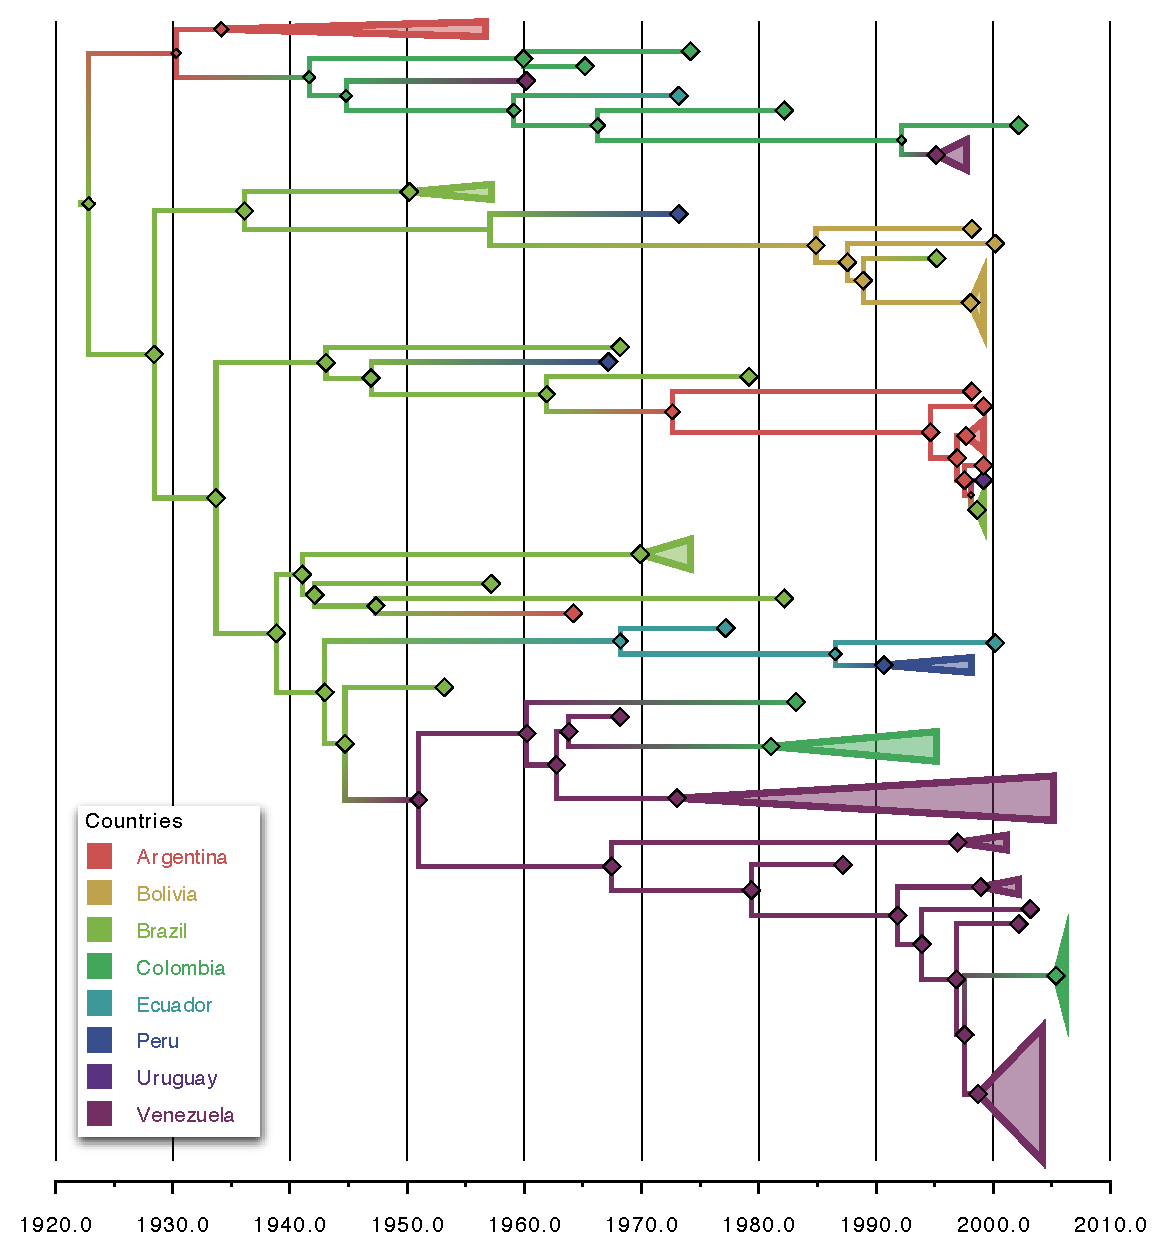
\includegraphics[width=\textwidth, height=10cm]{FIGURES/A.pdf}}\\
\subfigure[O]{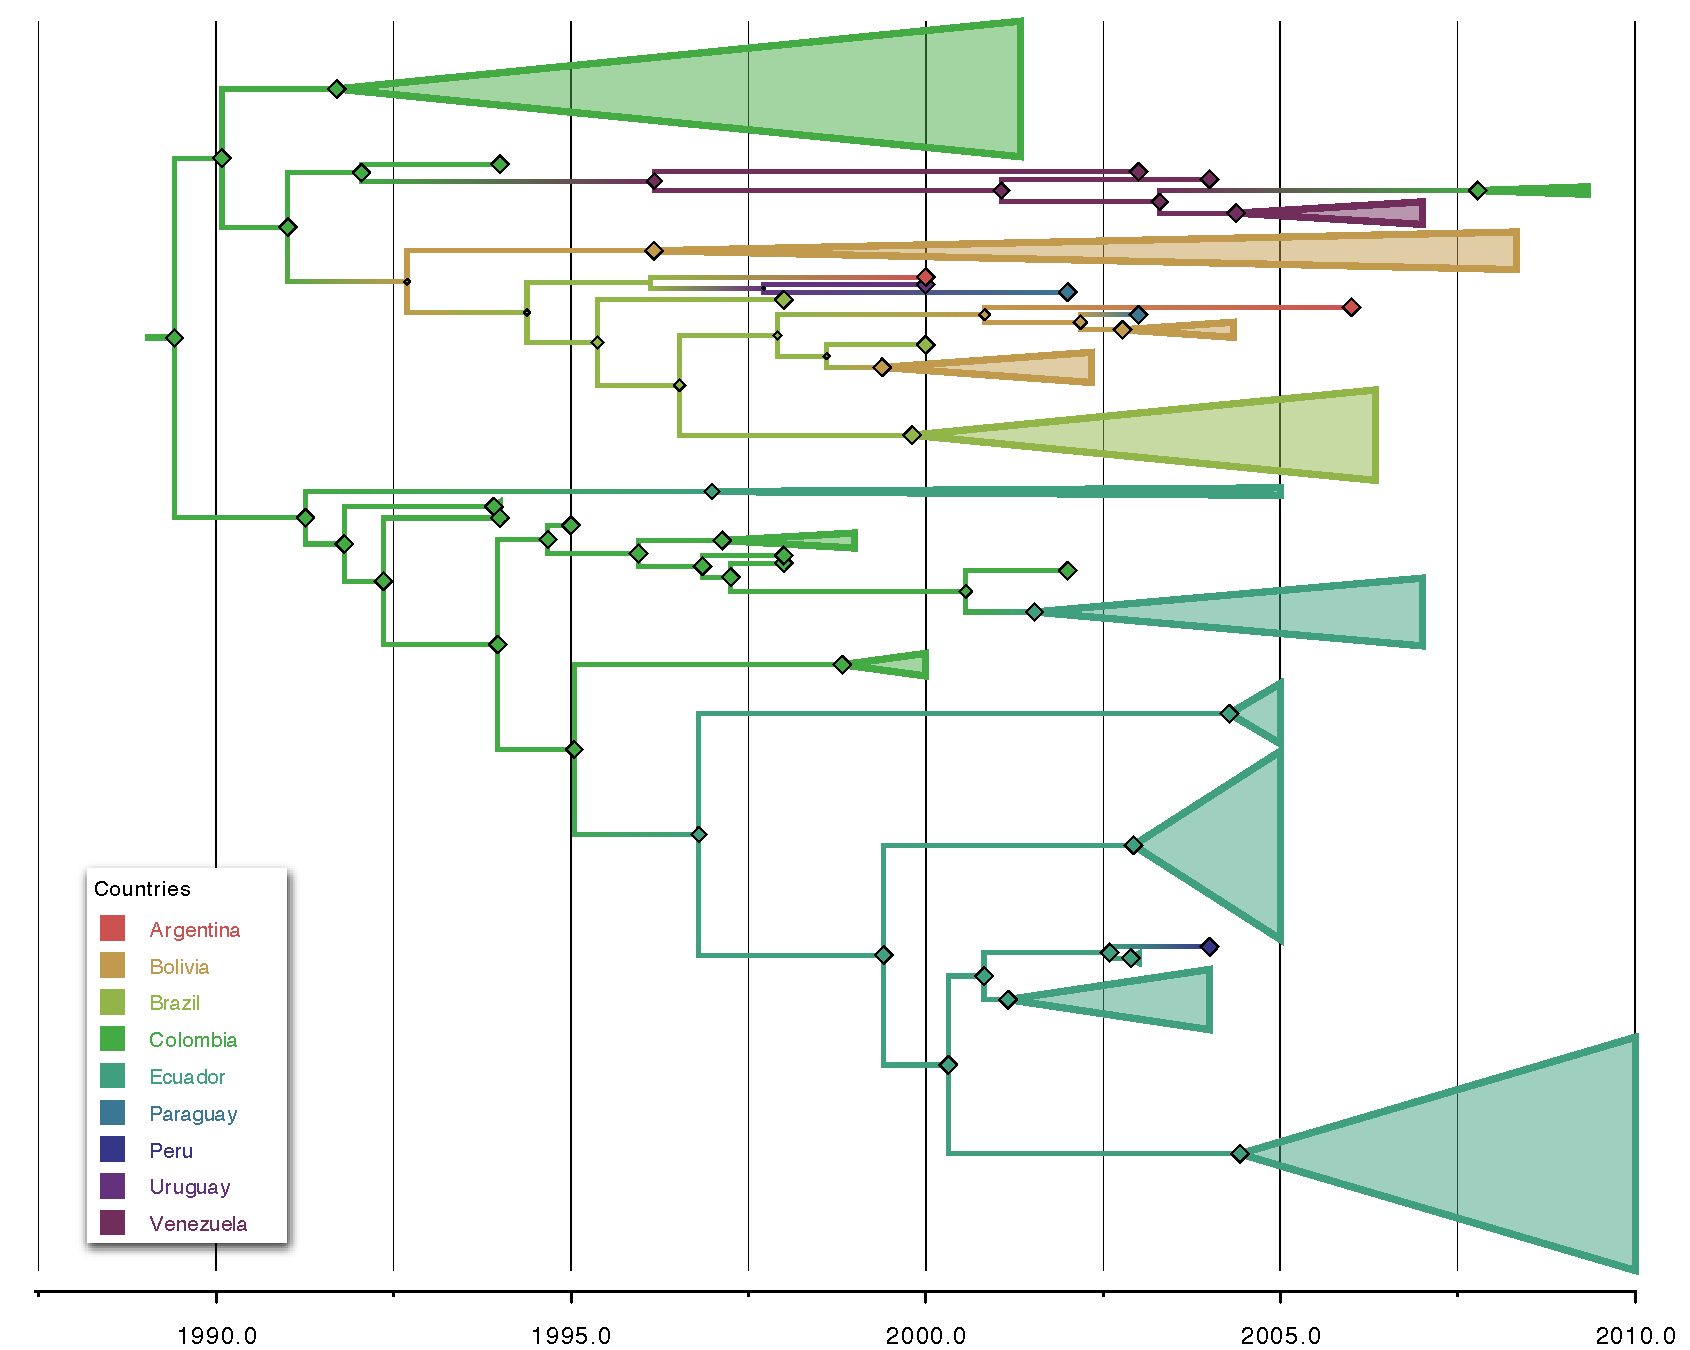
\includegraphics[width=\textwidth, height=10cm]{FIGURES/O.pdf}}
\end{center}
\caption{}
\label{fig:trees}
\end{figure}
%%%%%%%%%%%%%%%%%%%%%%%%%%
%%%%%%%%%%%%%%%%%%%%%%%%%%
\newpage
\begin{figure}[!ht]
\begin{center}
\subfigure[A --1945 ]{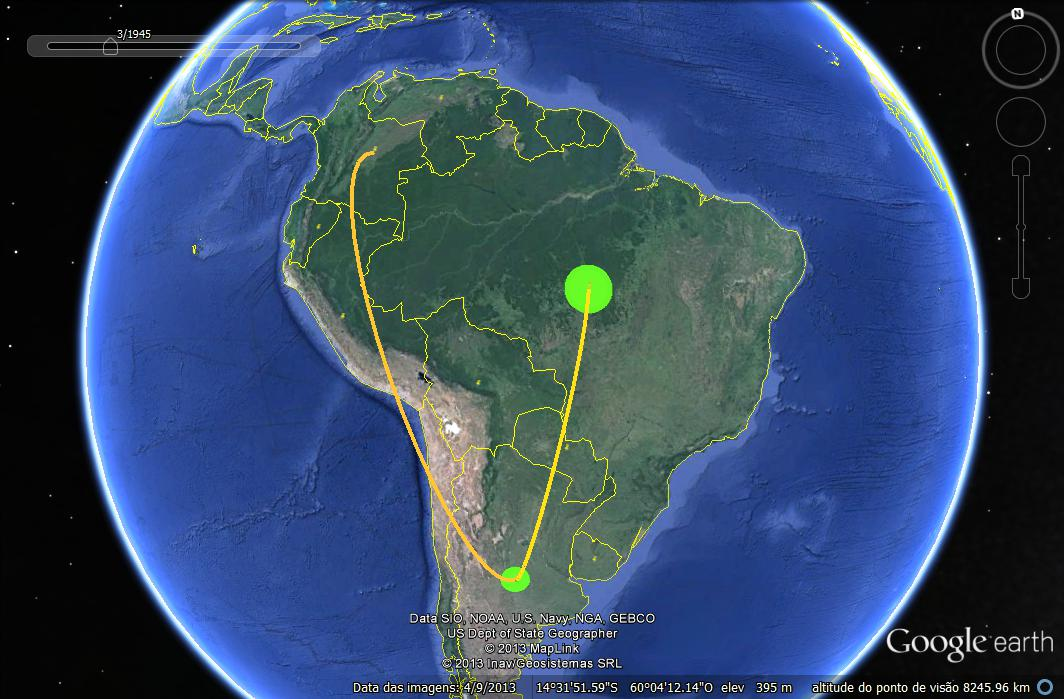
\includegraphics[scale=.20]{FIGURES/A_1945.jpg}}
\subfigure[O --1995 ]{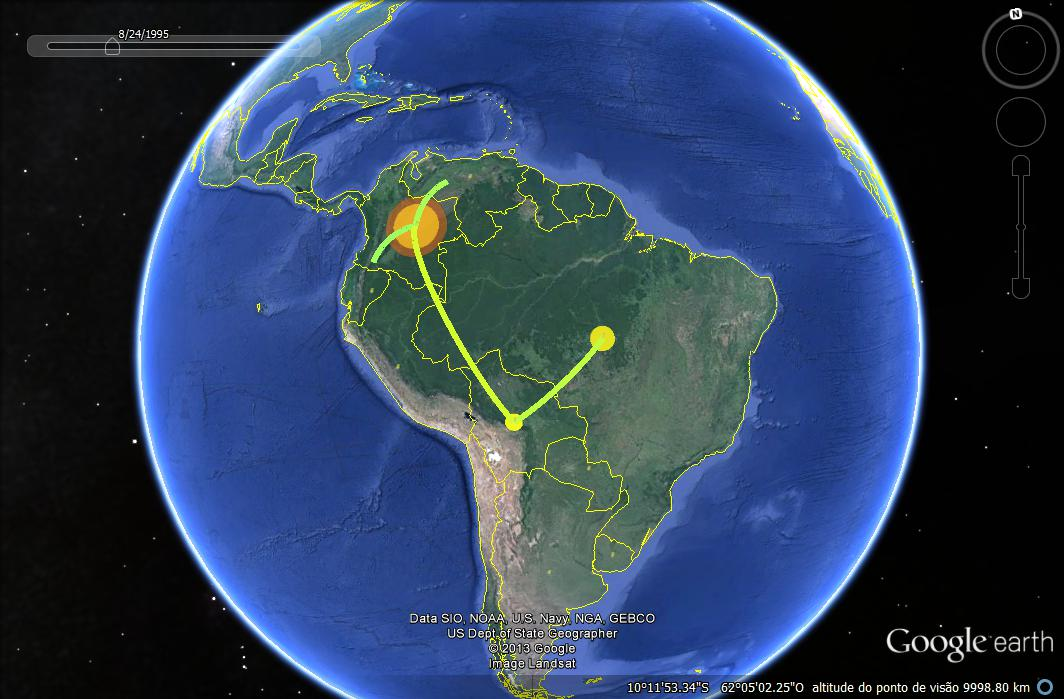
\includegraphics[scale=.20]{FIGURES/O_1995.jpg}}\\
\subfigure[A --1965 ]{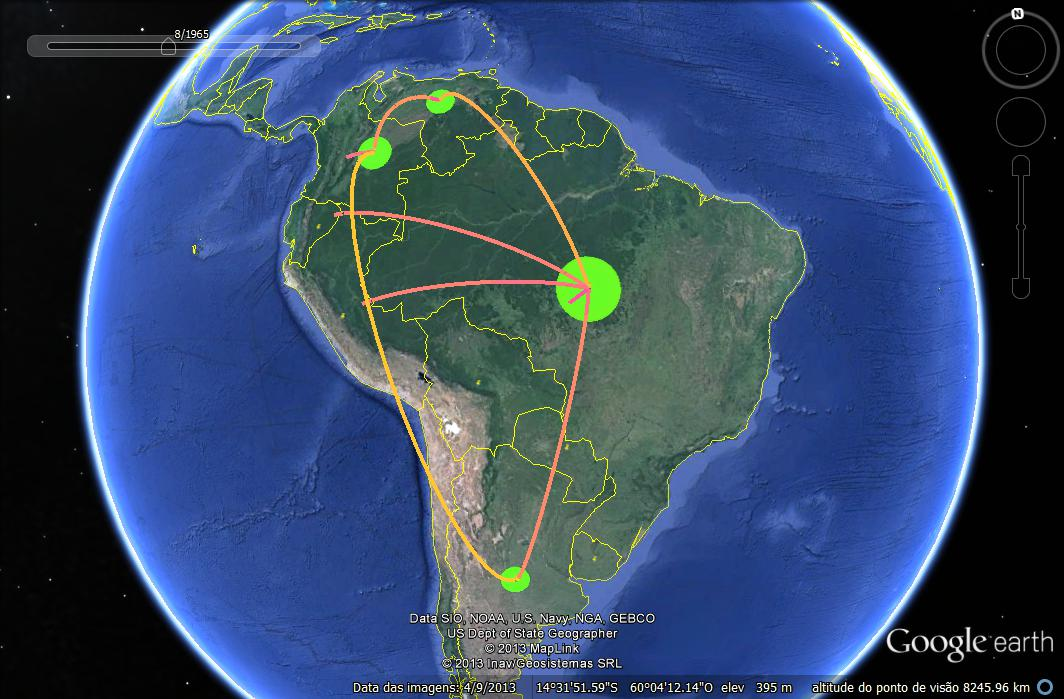
\includegraphics[scale=.20]{FIGURES/A_1965.jpg}}
\subfigure[O --2000 ]{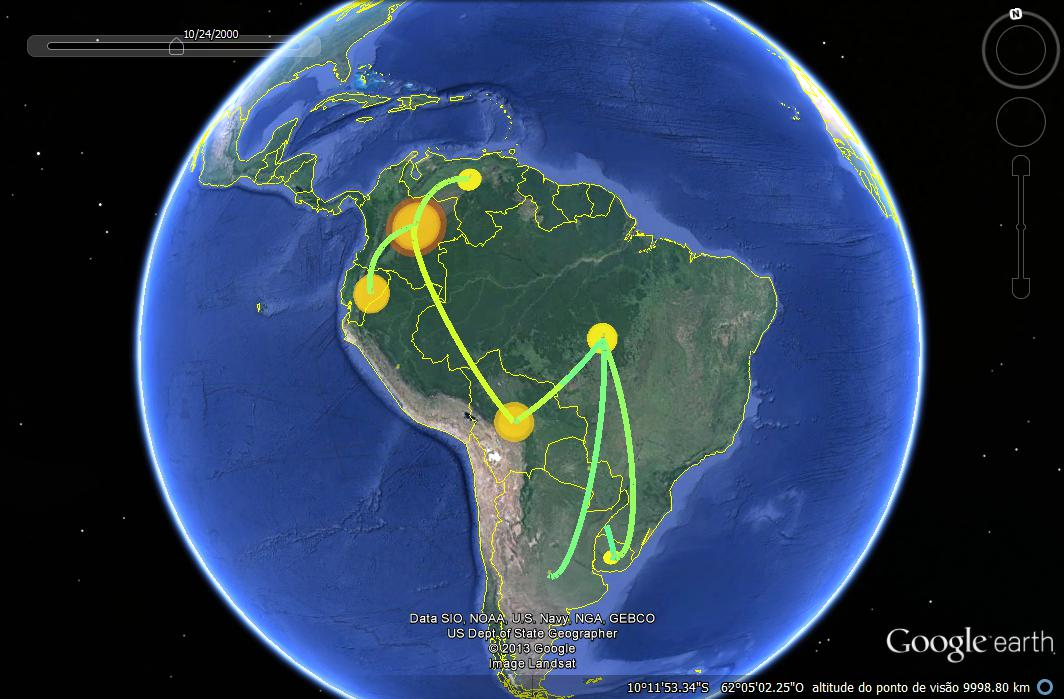
\includegraphics[scale=.20]{FIGURES/O_2000.jpg}}\\
\subfigure[A --1980 ]{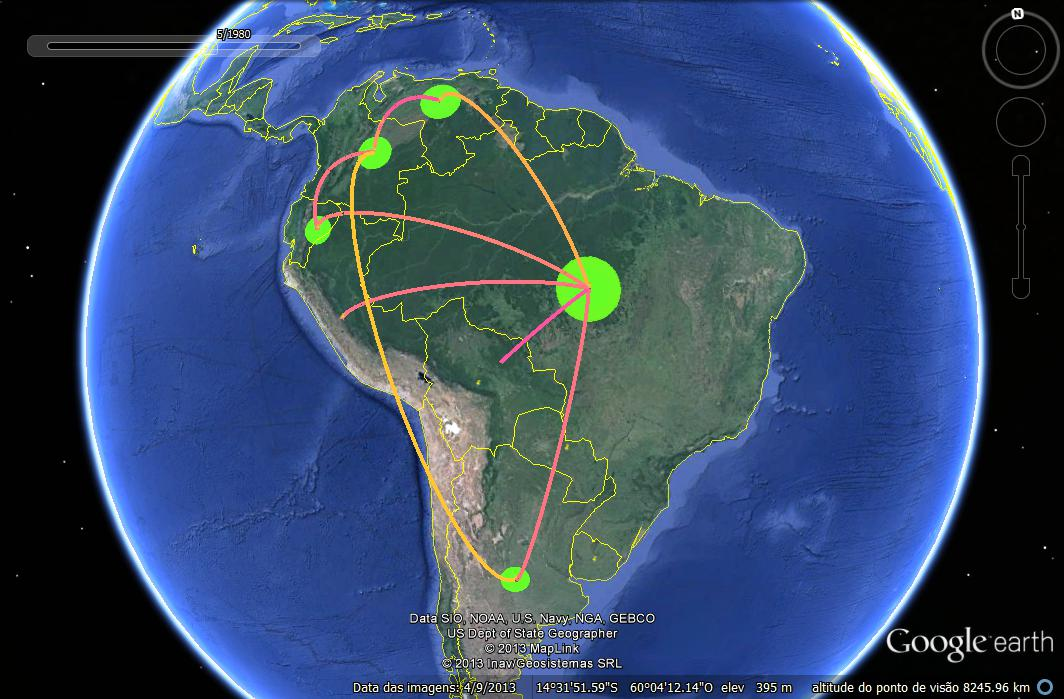
\includegraphics[scale=.20]{FIGURES/A_1980.jpg}}
\subfigure[O --2005 ]{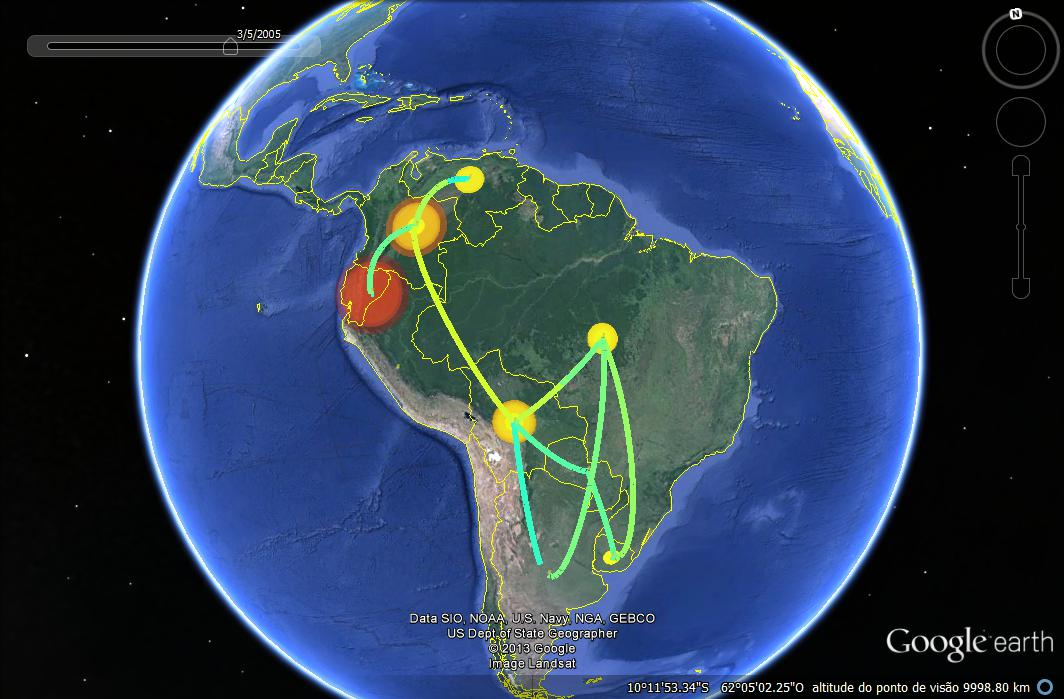
\includegraphics[scale=.20]{FIGURES/O_2005.jpg}}\\
\subfigure[A --2008 ]{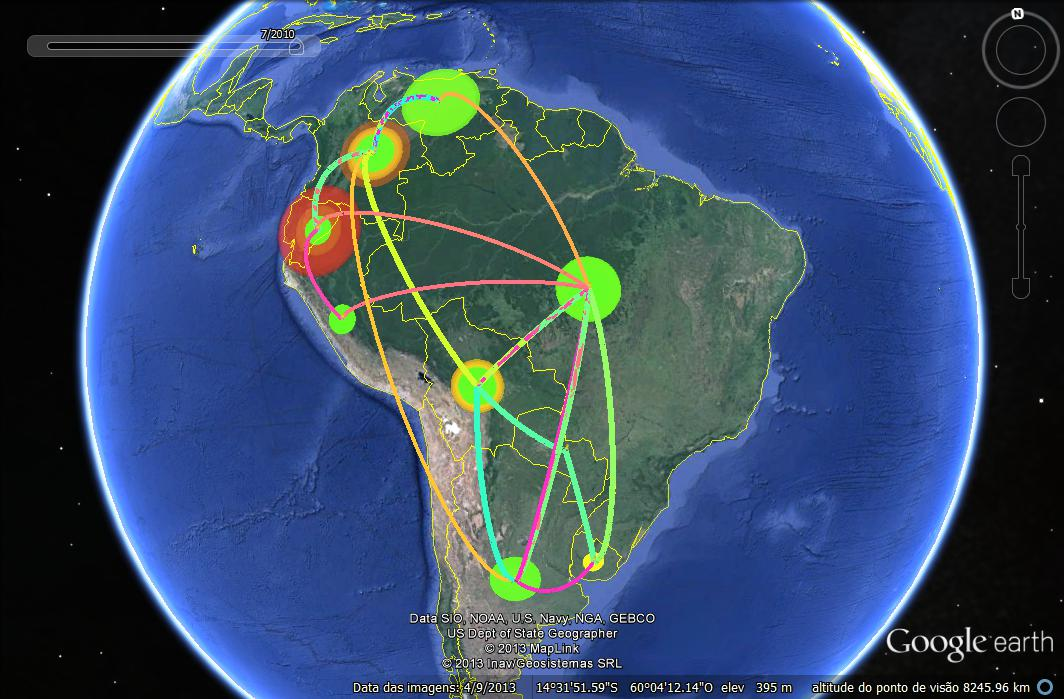
\includegraphics[scale=.20]{FIGURES/A_2008.jpg}}
\subfigure[O --2010 ]{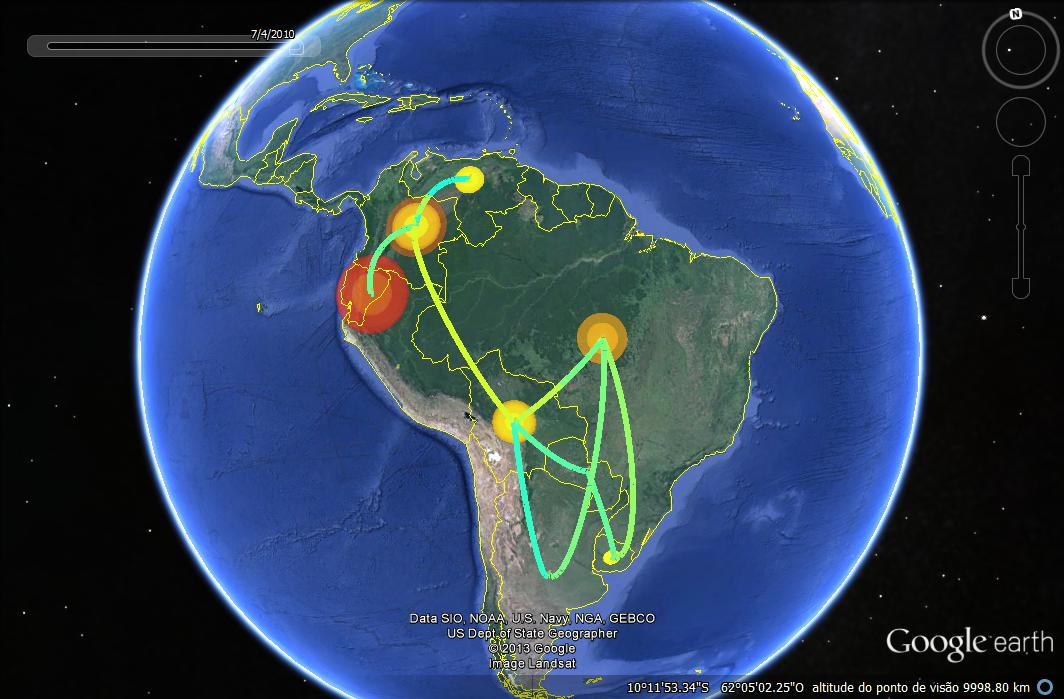
\includegraphics[scale=.20]{FIGURES/O_2010.jpg}}
\end{center}
\caption{}
\label{fig:migration}
\end{figure}
%%%%%%%%%%%%%%%%%%%%%%%%%%
%%%%%%%%%%%%%%%%%%%%%%%%%%
\newpage
\begin{figure}[!ht]
\begin{center}
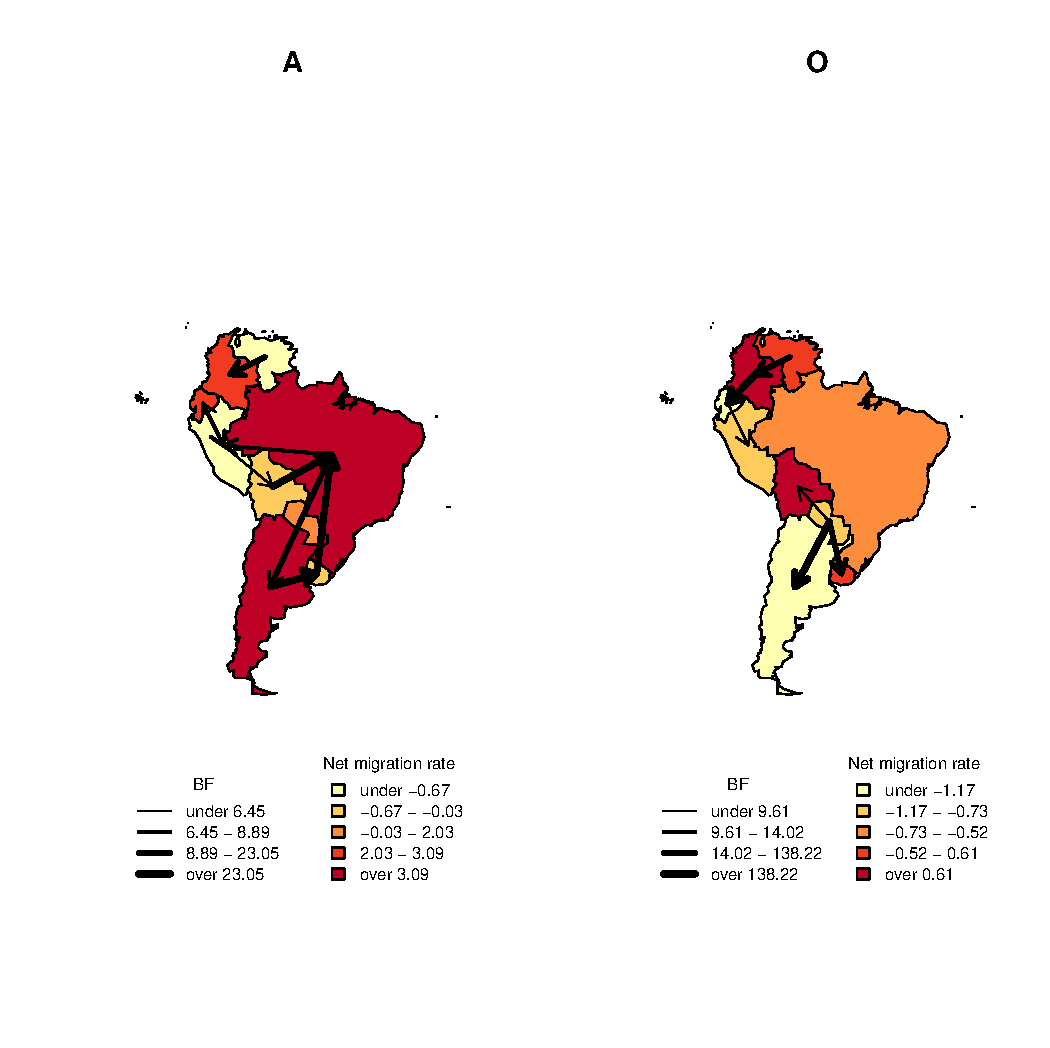
\includegraphics[scale=.85]{FIGURES/compound.pdf}
\end{center}
\caption{}
\label{fig:mj&BFs}
\end{figure}
%%%%%%%%%%%%%%%%%%%%%%%%%%
%%%%%%%%%%%%%%%%%%%%%%%%%%
\newpage
\begin{figure}[!ht]
\begin{center}
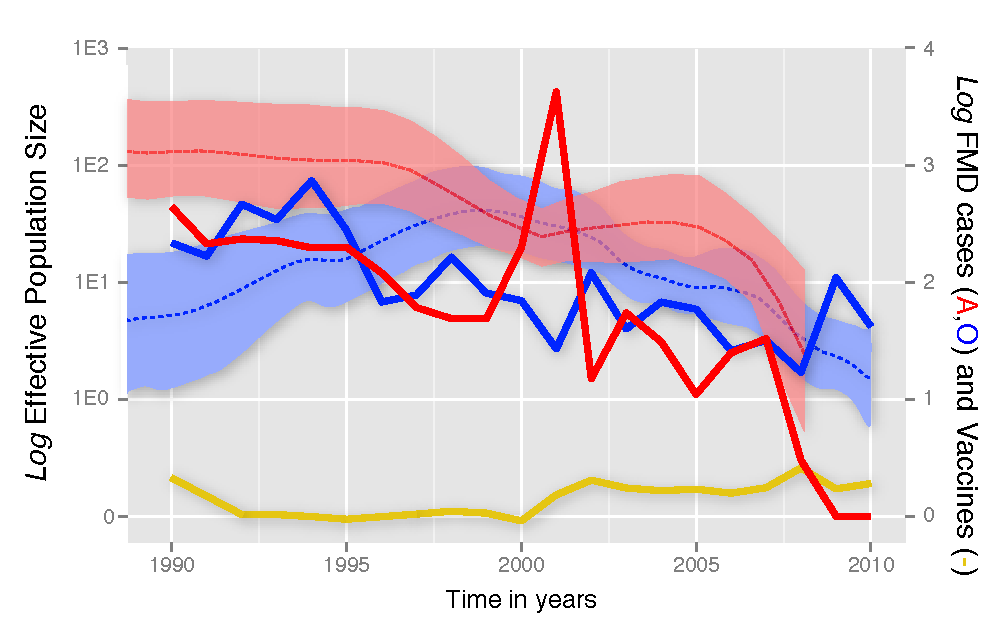
\includegraphics[scale=1.0]{FIGURES/skyride.pdf}
\end{center}
\caption{}
\label{fig:skyride}
\end{figure}
%%%%%%%%%%%%%%%%%%%%%%%%%%
%%%%%%%%%%%%%%%%%%%%%%%%%%
\newpage
\section*{Tables}
\begin{table}[!ht]
\caption{{\bf Comparison of combined and separate models for CTMC rate matrix} We calculated marginal likelhihoods for ``Shared'' and ``Separate'' models (see Methods). We present results obtaining by collecting different numbers of sample per ``step'' in Path Sampling (PS) and Stepping Stone Sampling (SS) algorithms.}
 \begin{center}
 \begin{tabular}{ccccccc}
 \toprule
 &\multicolumn{2}{c}{Shared}& \multicolumn{2}{c}{Separate} & \multicolumn{2}{c}{Bayes Factors}\\
 \midrule
Chain length & PS & SS & PS & SS & BF -- PS & BF -- SS \\
250k & -21420 & -21437 & -21436 & -21454 & 15.36 & 17.25 \\
500k & -21442 & -21456 & -21450 & -21467 & 8.00 & 11.00 \\
1M & -21462 & -21470 & -21471 & -21483 & 9.43 & 13.04 \\
% New 500K runs with uniform prior on Q
% SS-shared= -21431; SS-separate= -21449
\bottomrule
 \end{tabular}
 \end{center}
 \begin{flushleft}
\end{flushleft}
\label{tab:sharedsep}
\end{table}
%%%%%%%%%%%%%%%%%%%%%%%%
%%%%%%%%%%%%%%%%%%%%%%%%
\begin{table}[!ht]
\caption{
\textbf{Spatial model selection results for livestock predictors.} We assessed the significance of livestock trade in FMDV spread in South America using two importance sampling methods, i.e. path sampling (PS) and stepping-stone sampling (SS), to estimate (log) marginal likelihoods for each predictor using 64 path steps and 2 million iterations per path step. For each livestock predictor, we have tested equal location frequencies as well location frequencies equal to the proportion of that location's presence in the data set. We also present the (log) marginal likelihood estimates for two location priors under which the location rates are estimated, rather than being fixed (as for the livestock predictors). We put these two scenarios in a separate part of the table to indicate that these estimates should not be compared to those of the livestock predictors.}
\begin{center}
\begin{tabular}{llrrrrrr}
\toprule
 & & \multicolumn{3}{c}{Serotype A}& \multicolumn{3}{c}{Serotype O}\\
 \midrule
Predictor & Frequencies & PS & SS & BF$^2$ & PS & SS & BF \\
\hline
Cattle & Equal & -12608.72 & -12611.00 & -17 & \textbf{-8310.22} & \textbf{-8311.81} & 6 \\
Cattle & Sampling & -12661.11&-12663.11& -69 & \textbf{-8309.38} & \textbf{-8310.52} & 8 \\
Pigs & Equal & -12591.44 & -12591.64 & 2 & -8329.98 & -8332.00 & -14 \\
Pigs & Sampling & -12644.69 & -12645.95 & -52 & -8338.54 & -8338.16 & -20 \\
Sheep & Equal & \textbf{-12572.09} & \textbf{-12573.78} & 20 & -8323.22 & -8323.68 & -5 \\
Sheep & Sampling & -12592.84 & -12594.05 & 0 & -8328.65 & -8330.90 & -13 \\
\hline
Distance & Sampling & -12587.78 & -12590.61 & 4 & -8315.07 & -8318.48 & 0 \\
Uniform & Sampling & -12590.92 & -12594.11 & - & -8314.47 & -8318.25 & - \\
\bottomrule
\end{tabular}
\end{center}
\begin{flushleft}
\end{flushleft}
\label{tab:preds}
 \end{table}
%%%%%%%%%%%%%%%%%%%%%%%%
%%%%%%%%%%%%%%%%%%%%%%%%
\begin{table}[!ht]
\caption{
\textbf{Inferred root locations for each predictor for both serotypes.} We present most probable country of origin inferred using each predictor, with associated probabilities inside parentheses. 1- Uniform, all rates equal prior.
}
\begin{center}
\begin{tabular}{lcc}
\toprule
Model & Serotype A & Serotype O \\
\midrule
Distance & Peru (0.96)& Colombia (0.92)\\
Sheep    & Brazil (0.90) & Colombia (0.98)\\
Pig      & Colombia (0.99) &Colombia (0.52)\\
Uniform$^1$  & Peru (0.96) &Colombia (0.92)\\
Cattle   & Peru (0.94) &Colombia (0.95)\\
Sheep-Freq & Peru (0.84)&Colombia (0.86)\\
Pig-Freq & Colombia (0.72) &Colombia (0.71)\\
Cattle-Freq & Peru (0.92)& Colombia (0.97)\\
 \bottomrule
\end{tabular}
\end{center}
\begin{flushleft}
\end{flushleft}
\label{tab:roots}
 \end{table}
%%%%%%%%%%%%%%%%%%%%%%%%
%%%%%%%%%%%%%%%%%%%%%%%%
\end{document}
 

\bibliographystyle{mbe}

\begin{letter}{
	Dr. Santiago F. Elena\\
    Editor-in-Chief \\
    Virus Evolution
}

%----------------------------------------------------------------------------------------
%	LETTER CONTENT
%----------------------------------------------------------------------------------------

\opening{Dear Dr.~Elena,}

I would like to submit the manuscript entitled ``Spatio-temporal Dynamics of Foot-and-Mouth Disease Virus in South America" for consideration for publication in \textit{Virus Evolution}.

This manuscript was originally submitted to~\textit{Virus Evolution} in 2015 and was assigned manuscript ID VEVOLU-2015-010. 
After the first round of revisions, I was unfortunately unable to perform the extensive modifications requested by the referees.
After concluding my PhD in 2019 I was able to return to this project and re-collect and re-analyse the data using a better analytical framework that accounts for collection (sampling) bias explicitly, including the techniques in~\cite{Karcher2020} .

It is  our understanding that the manuscript brings a substantial methodological advance that sheds light into the dynamics of an important livestock virus at a continental level -- previous analyses have been restricted to single countries (e.g. Ecuador and Argentina) or regions (e.g. Andes).
Thus, we consider the manuscript to be of interest to the readership of~\textit{Virus Evolution} both from a methodological and an applied point of view.

As an appendix to this letter I provide a point-by-point response to each point by each reviewer clarifying the improvements made.
In providing our revision, we have carefully considered the helpful suggestions and critiques of yourself and three Reviewers.
You will find a point-by-point response (bold) to all comments (normal text) we received.
Significant changes to the manuscript find themselves in quotes.

\closing{Sincerely,}

\clearpage

%====================
\textbf{Editor-in-Chief}
%====================

Dear Mr. Carvalho,

Manuscript ID VEVOLU-2015-010 entitled ``Spatio-temporal Dynamics of Foot-and-Mouth Disease Virus in South America'' which you submitted to Virus Evolution, has been reviewed.  
The comments of the reviewer(s) are included at the foot of this letter.

The three reviewers have very diverse opinions, from rejection (2nd reviewer) to minor revisions (3rd reviewer), thus the decision cannot be other but to request you to perform a major revision.  
Therefore, I invite you to respond to the reviewer(s)' comments and revise your manuscript.  
Please notice that given the nature of these comments and of the required amount of modifications, the new version will be send out for a second round of review, most likely to the same reviewers.

Once again, thank you for submitting your manuscript to Virus Evolution and I look forward to receiving your revision.

Sincerely,
Dr. Santiago Elena
Editor-in-Chief
Virus Evolution

\begin{reply}
We thank the Editor-in-Chief and agree that the Reviewers' comments have helped us improve our manuscript. 
As the referees shared some of the same concerns, we address those in general comments.
\end{reply}


\textbf{General comment \#1: New data}

\begin{reply}
A major criticism of our original submission was that we did not use all of the publicly available data.
To address this we conducted a through search of GenBank, now described in the Methods section of the paper:
\begin{quote}
We retrieved all FMDV nucleotide sequences available from GenBank~\citep{Benson2013} from the National Center for Biotechnology Information (NCBI, \url{ http://www.ncbi.nlm.nih.gov/}) with more than $600$ bp.
This first step yielded $6, 907$ sequences which were then filtered to exclude all sequences that did not include the 1D (VP1) gene, resulting in $4, 507$ sequences being kept.
We then filtered for sequences from serotypes A and O, yielding $1051$ and $2350$ sequences, respectively.
Next, we excluded sequences that had been extensively passaged in cell culture and selected all sequences from South America (Argentina, Bolivia, Brazil, Colombia, Ecuador, Paraguay, Peru, Uruguay, Venezuela) for which information on country and year of isolation was available.
\end{quote}
This procedure lead to $53$ additional sequences for serotype A and $43$ sequences for serotype O. 
\end{reply}


\textbf{General comment \#2: Accommodating temporal and spatial sampling bias}

\begin{reply}
Even with broader sampling, the use of observational data brings with it the concern that temporal and spatial sampling bias might lead to incorrect inferences.
We address this important concern by employing analytical methods that explicitly accommodate the possibility of sampling bias.

On the temporal side, we employ the modelling framework of~\cite{Karcher2020} to fit various coalescent-based models that specify the dependence of the sampling process on the population size or other temporal factors, while also accounting for phylogenetic uncertainty.
Using with marginal likelihoods, we can compare these models and infer not only whether there is significant temporal bias but also possible explanatory factors.

To account for spatial bias, we employed a general linear model (GLM)~\citep{Lemey2014,Dudas2017} that allows for several predictors of spatial spread to be included simultaneously.
This has the benefit of allowing one to construct predictors that account for possible sampling bias, such as the difference in numbers of sequences between locations and also the numbers of sequences at both origin and destination.
By assessing the posterior inclusion probability of these sampling bias proxies, we can assert whether they contribute significantly to estimated dispersal rates.
This framework also allows consideration of further predictors~\textit{in addition to} the sampling bias ``controls''.

In summary, we have updated the statistical methods in the paper so as to accommodate and test for sampling bias.
It should be noted, however, that these methods are not a silver bullet; a biased sample will always be a biased sample and inferences will be affected regardless.
The use of principled statistical methods helps mitigate the bias and uncover the true patterns in the data.
\end{reply}

%====================
\textbf{Reviewer \#1}
%====================

The manuscript by Carvalho et al., describes the analysis of foot-and-mouth disease viruses (FMDVs) of two different serotypes (O and A) based on partial genome sequences from samples collected during a 55 year period for serotype A and 16 years for serotype O. 
The sequence analysis data is linked to studies on the trade of FMDV susceptible animals, e.g. cattle and pigs. 
The study has some interest but from my point of view, there seem to be some surprising omissions of information which may, or may not, affect the conclusions that can be drawn.

Specific points

1)      In the Abstract, the text indicates that serotype O emerged (in South America) in around 1990. 
This is an odd statement to make since there are well known FMDV serotype O strains that predate this, e.g. O11 Campos (from Brazil in 1958), O1 Argentina (c. 1965) and O/M11/MEX from Mexico in 1952 which have all been sequenced in part and accession numbers are available (cited in Wright et al., (2013) Infect Genetics Evolution 20, 230-238).  
How does consideration of such sequences influence the information about the date of introduction of the viruses and their circulation in South America? 
In the Introduction, the authors indicate that: ``Historically, serotype O has been the most prevalent serotype on the continent''? (lines 53-55, P1). 
The authors need to explain why the earlier strains of FMD virus were not included in their analyses.

\begin{reply}
We thank the reviewer for catching this.
Firstly, the Mexico sample(s) was not included because we chose to restrict attention to South America.
Secondly, we updated our data sets to include many more sequences.
Please see General Comment \#1 for more information.
\end{reply}

2)      It is curious that there is no mention of serotype C FMDV in South America.

\begin{reply}
Serotype C was indeed mentioned in the introduction (line 55): ``Serotype C on the other hand was last encountered in the continent in 1995 in Brazil'' .
\end{reply}

3)      The sequence analysis is based on the VP1 coding region, this only represents about 630 nt out of a complete FMDV genome of about 8400nt. 
This information is not presented within the Introduction or Results section of the manuscript and only becomes apparent from Figure legends and Material \& Methods (i.e. it is quite well hidden). 
The resolution of the analyses based on VP1 coding region sequence information alone is necessarily limited. 
Full genome (or near full genome) sequencing can give much higher resolution, e.g. to the level of farm-to-farm spread (e.g. see Valdazo-Gonzalez et al., (2012) PLosOne 7(11) e49650).

\begin{reply}
The fact that we use VP1 sequences is explicit in the methodology and all of our data and code are publicly available.
In any case, we have now added a whole section at the end of the paper called ``Limitations of this study'' to address concerns of partial versus full genomes, which we agree is an important caveat.
We have also included a citation of Valdazo-Gonzalez et al., (2012) in our discussion of full genomes~\textit{versus} partial sequences.
\end{reply}

4) The nature of the samples used for the virus sequence determination is also not indicated, have some been extensively passaged in cell culture? 
This information should be available using the accession numbers of the published sequences and clearly can influence the outcome of sequence comparisons.

\begin{reply}
We excluded sequences coming from samples that had been extensively passaged. 
The Supplementary Material includes a list of all sequences used, as well as those excluded based on this and other criteria. 
\end{reply}

5) I am not familiar with the ``root-to-tip'' plots shown in Figure S1 but it seems to me that the slope of the line for serotype A over the period from 1995 to 2010 is not very different from that of serotype O over this limited time period and is rather different from that for the whole time period for serotype A. 
It would be useful if the authors commented.

\begin{reply}
The slope in a root-to-tip regression is a rough estimate of the evolutionary rate, and in this case both serotypes have markedly different evolutionary rates.
At any rate, since the data sets have substantially changed, so have the plots.
\end{reply}

6)      A major concern about identifying origins of samples is having adequate coverage of samples from potential sources. 
It is not entirely clear to me that the coverage of FMDV strains circulating in South America is sufficient to be able to draw good conclusions. 
It may be that it is but this is not clearly demonstrated.

\begin{reply}
Please see General comment \#1.
\end{reply}

7)      On P.4, lines 48-50. The text indicates that the importance of long range migration routes seems to differ for the two serotypes but the confidence values for the two serotypes seem to overlap extensively, so is this a real difference?

\begin{reply}
We thank the reviewer for catching this.
We have now removed this analysis as it did not address the epidemiological question appropriately.
We now limit our discussion to qualitative observations of well-supported (BF $>3$) long-range migrations for both serotypes without attempting a quantification. 
\end{reply}

8)      Recombination within the coding region for VP1 alone is rather rare and thus I am not sure the check for recombination was very justified or useful (P. 9 lines 8-11).

\begin{reply}
We have removed this analysis.
\end{reply}


%====================
\textbf{Reviewer \#2}
%====================

Comments to the Author
The ``Spatio-temporal dynamics of FMDV in South America'' study by Carvalho et al. describes the historical spatio-temporal dispersal of FMDV across the South America continent reconstructed using phylogeography analyses employed through a Bayesian spatial diffusion model. 
The reported results define transmission networks and transmission hubs (at country level) that would explain the historical spread of FMD within the continent. 
In addition, the authors deal with variables likely associated with the FMD spread (i.e. geographical distance, livestock density, and livestock trade) in trying to explain their causative effect associated with historical FMD outbreaks. 
As last attempt, the authors correlated the demographic dynamics of FMDV with reported number of FMD outbreak and vaccination coverage in trying to assess the impact of FMD control policies on the FMDV diversity and its population expansion/contraction through time. 
The paper has been already published as an arXiv (http://arxiv.org/abs/1505.01105) the 5th of May. 
Although the methodological approach has been previously used in different setting and the results would be interesting for a computational basis, there are several aspects of the study that need to be carefully considered before the paper would be suitable for publication. 
In fact, the presence of bias in the data used is potentially producing an incorrect picture of FMD in South America. 
In addition, although the authors are examining the potential impact of the sampling bias in the sequence data analysed, this is only properly discussed as Supplementary Text and not in the main paper, where they assume the results as correct, valid and without bias. 
One major problem of the study is the data. 
They claim to have analysed all the data publicly available in GenBank but (as detailed below) this is not correct and the analyses should be repeated including the full sequence dataset. 
I would be, therefore, really cautious to draw important conclusion from this study given the issues reported, which might hold true only for the time-frame pictured from the data you have analysed. 
As already said, this study need a proper revision before being published and this main revision would involve the re-analysis of all the data adding all the sequences available in GenBank and which are not included in this version.

\begin{reply}
We thank the reviewer for such a through assessment of our work.
It seems the reviewer's main concerns were (i) incomplete sampling of available data; (ii) sampling bias (even in face of all available data) and (iii) the level of generality of the results in face of (i) and (ii).
We have now re-done the data collection and improved the data sets we analyse.
We also employ better models that account for sampling bias both in time and space.
For more please see responses below and also General Comments \#1 and \#2.
\end{reply}

Problems of the study:
-       The authors claim to have used all publicly available VP1 sequences from GenBank, but after inspection this is not true. 
In fact, there are quite a number of sequences that has not been included in the study. If this has been done intentionally, the reason for this decision should be discussed in the paper; if not, I strongly suggest checking better in GenBank what is missing from your analyses (you have even the GenBank Accession Nos of the missing data in one of your reference [Malirat et al., 2007]). 
For the serotype O, for example, you are totally ``ignoring'' the sequences before the 1994 but, what about the O/Campos (O/Br/58) and the Argentinian samples of the 82-83 or the Caseros/67, the Selab/77? I could make the list much longer. 
This is valid for the serotype A as well (e.g. among others, where is the A10/Arg/61?). 
Therefore, if you want to claim to have analysed the complete VP1 coding sequence data for South America you need to re-perform all the analyses, because the results might provide you a completely different picture of FMD in South America (see your conclusion on the Colombian origin of the type O in South America).

\begin{reply}
We thank the reviewer for their careful assessment of our data.
It is indeed true we had not included many sequences that could otherwise have been analysed.
This has now changed and we have collected $53$ additional sequences for serotype A and $43$ sequences for serotype O (See General Comment \#1).
\end{reply}

-       All the results discussed on the spatial diffusion of FMDV in the whole South America continent should be treated with cautions (potentially providing you incorrect data), considering that you have: missing information from missing sequences; a sampling bias in your data according to time and country. 
It is well known that FMDV was introduced (as you pointed out in the introduction) by human migration from Europe in the end of the 19th Century with early reports in Argentina between 1860 and 1870, and 1895 in Brazil. 
There were at least two distinct introductions in the North and one in the South but, before the 1922, it is really difficult to say which serotype was (i.e. before the FMDV typing was performed). 
However, it is clear that the early spread of FMD was coming from the South. 
Argentina at the time was one of the main export hubs of livestock to the continent and even the Mexico outbreak in 1922 has been attributed by the introduction of infected cattle from Argentina. 
This holds true for: Chile, 1920 outbreak (decline of cattle industry during 1912 in Chile with large introduction from Argentina); official report in Venezuela 1950 (potential from importation of Argentinian meats/livestock back to the 1947). 
It might worth to know that the Andes acted as a barrier for taking FMD out of Chile and the western part of South America, until when the regional animal movements and trade primarily caused the spread. 
The countries of the Rio de la Plata, which were sharing the Pampas ecosystem, experienced an early wave of disease spread and by the 1920 FMD was in Uruguay, Paraguay and Brazil. 
Historical data suggest that type O was introduced most likely from the South (maybe Argentina) and type A introduced from Europe. 
From your analysis the initial historical FMD wave has not been characterised (in the years before 1994 for type A; very limited and potentially biased before 1965 for type O). 
The only part which might be more realistic is the FMD transboundary movements within the ``countries triangle'' of Colombia, Ecuador and Venezuela, that could sounds more like from Argentina-Venezuela-Colombia-Ecuador, even though you have the effect of sampling bias that needs to be discussed.

\begin{reply}
We share the reviewers concerns that sampling bias might be an important factor in our analyses.
This has been addressed using state-of-the-art phylodynamic methods which accommodate both temporal and spatial sampling bias.
While not a panacea, these methods are the best one can do in face of incomplete and potentially biased data.
For more, see General Comment \#2.
\end{reply}

-       Although you presented some data on sampling bias in your Supplementary Text (but this might be not satisfactory enough given the problem in the dataset), there is a real problem of sampling bias and this need to be addressed in your main text as well. 
How does the model deal with missing links? 
Is the prediction robust enough to provide a clear indication of virus spread in such a large geographical range? 
This could be a serious limitation (and problem) of your study. For serotype A, you analysed 131 VP1 sequences of which 44\% are from Argentina (of which $\sim$70\% are from 2000 and 2001) and 21\% from Venezuela (of which $\sim$86\% are recent samples - after 2001). 
In addition, the majority of your oldest samples are only from Brazil and Argentina. For serotype O, you have 167 sequences in total of which $\sim$54\% are from Ecuador (all after the 2002 and have been previously analysed - along with 30 sequences that have been included in this manuscript as well). 
Therefore, you have 90+30=120 sequences already analysed in a previous paper. 
Among the other, 36 sequences from Colombia ($\sim$22\% of the total) are barely covering the 2000s (as you claim 1994 to 2008), since you have 5 sequences from 2000, 1 from 2002 and 2 from 2008, a gap of 6 year. 
For the type A database, your oldest samples are only from Colombia. You attempted a random sub-sampling that, as far as I understood, have not taken into account the time of sampling, but just the quantity of data from each country. 
Maybe you need to account for time in your sub-sampling.

\begin{reply}
We now consider a model that explicitly accounts for temporal biases in the sampling process. 
\end{reply}

-       When doing analysis on sequences extracted from GenBank a detailed list of the sequences with their GenBank Accession No (along with associated metadata) should always be provided. 
Although a webpage (but this is difficult to check and, probably, the majority of the readers would not bother to access to your website) has been set up for the paper there are no GenBank references for the serotype A. 
This information should be included either as a table in the main text or as a S3.

\begin{reply}
This list is now available from the PDF of the Supplementary Material.
\end{reply}

-       This paper has been already published as an arXiv (http://arxiv.org/abs/1505.01105) which has been submitted the 5th of May and updated the 2nd of June (I received this review the 12th of June). 
Although it is common for theoretical maths, physics and computer sciences studies to be published as arXiv before being properly peer-reviewed, this is not the case with study dealing with topics as in this case. 
Since the study needs a substantial review and re-analysis of the data, I would suggest to withdraw your submission to arXiv

\begin{reply}
This comment makes no sense in light of the journal's policy.
\end{reply}

Major Comments:
-       Page 1 Line 36: ``Our dating''. 
This result is only compatible with your dataset and must not be related with the incursion of FMD in South America. 
Your dating is referred to the MRCAs of the data you have analysed but not the MRCAs of both the type A and O clades in South America. 
As already detailed the occurrences of both serotypes are much earlier than your estimates, which therefore are misleading in the description. 
If you comment on the South America FMD phylogenetic history, you need to do that only in line with the data you analysed and not as a general picture.

\begin{reply}
Whilst the occurrence of both serotypes might have occurred much earlier than the estimates we obtain, the estimates are for the origin of the~\textit{circulating} strains.
It is entirely possible FMDV has been introduced several times in South America.
\end{reply}

-       Page 2 Line 7: ``By the 1970s''. 
Again this is not true. 
During 1950s FMD was already causing problems in Argentina, Brazil, Chile, Peru, Uruguay, Venezuela, Colombia, and Ecuador. 
This picture is larger than a regional scale.

\begin{reply}
``Causing problems'' is not the same as having widespread epidemics.
See the reference we give~\citep{Saraiva2003} for more details.
\end{reply}

-       Page 2 Line 33: ``using all''. 
You are not using all the sequences available in GenBank. 
For example and as already commented, I cannot find the O Campos in your fasta file (and this is only one). 
I strongly suggest doing a better search and re-perform all the analyses.

\begin{reply}
This has now been done.
\end{reply}

-       Page 3 Line 20: ``the time of the most recent''. 
You need to clearly state here that these estimates hold true only for your sequences analysed (MRCSs of the data) and not of the entire South America because saying that is misleading and incorrect.

\begin{reply}
We have now clarified that the estimates as presented pertain to the data set at hand.
\end{reply}

-       Page 3 Line 21: ``indicating a more recent origin''. 
Again this is only true for your data and should be stated. 
Serotype O outbreaks have been reported in South America since the initial wave, but clear reports start from 1940-50 (e.g. massive outbreak in Peru in 1962; 1950 official report in Venezuela; 1957 A, O and C in the entire Rio Grande do Sul).

\begin{reply}
Again, this is the origin of the circulating strains, which is all that can be said~\textbf{from any particular sequence data set}.
\end{reply}

-       Page 3 Line 22: the results show a faster clock for the type O than the A (even this is not really a lot faster - considering the VP1 only there is a difference between the two of $\sim$4nt changes per year). 
Might this be due to the different molecular clock model used for type A and O?

\begin{reply}
The difference is not due to the choice of model because we considered the same set of molecular clock models for both serotypes, selecting those that provided the best fit for each.
Rate estimates are, however, widely consistent across models, for each serotype.
\end{reply}

-       Page 4 Line 49: ``Remarkably''. 
You claim that there is a difference between long-range migration routes between serotypes (reported as 0.14 and 0.05 for type A and O, respectively). 
However, the 95\% intervals are really similar and both containing the zero, I should then say that this is not so remarkable.

\begin{reply}
This analysis has now been excluded from the manuscript.
\end{reply}

-       Page 4 Line 57: ``The most probable''. 
This result might indicate that the 2001 reappearance of FMDV in Argentina was a persistent virus foci (maybe carrier?) or maybe some missing links (i.e. sampling bias) exists in your data which are not including contemporary isolates from neighbouring countries (besides Brazil) and, therefore, this would impact on your results. 
Since this would be quite an interest topic (even though only on a retrospective line), you need to discuss this in more details, assessing as well the validity of your results.

\begin{reply}
Our GLM analyses attempt to account for sampling bias, and find only mild evidence of bias (BFs $<3$ indicate weak support, see Figure 5 in the revised manuscript). 
We have now expanded the discussion of these issues a little more in the revised manuscript.
\end{reply}

-       Page 5 results on the Venezuelan origin of Andean FMDV spread: 
Considering that you have a bias in your sequences for type A, you need to really consider with caution your results and discuss more about the impact it might cause.

\begin{reply}
The question of bias has been addressed more thoroughly (see General Comment \#2).
\end{reply}

-       Page 5 Line 16: ``Similar to what was found for Venezuela''. 
You present data on Colombia saying that this results is similar to type A for Venezuela? however, I would rather imagine that you are discussing about source of type O in the north from Colombia. 
Is this true? If so, please rewrite the sentence to make that clear. 
In addition, since you have all the oldest historical samples of type O from Colombia, the logical reasoning would be that of course the analysis point to Colombia as the main transmission hub. 
But, what about the sequences you have not included in the analysis? 
Should this provide you a different picture? 
You need to clearly discuss this issue (and of course re-perform the analysed including all the data available)

\begin{reply}
The discussion of the spatial origins results has now been completely re-written, among other reasons to accommodate the new sequences being analysed.
While common sense would dictate that the location with the oldest samples would be inferred as root, this is simply not true for the CTMC model we employ: the root state can potentially be any of the sampled states (countries).
\end{reply}

-       Page 5 Lines 34-38 and following paragraph (Lines 41-57): ``or serotype A''. 
This sentence is really confusing and need to be better formulated. 
For type A you find that geographical distance drives the diffusion, whilst this has a higher statistical support for type O but not like the cattle exchange. 
Now, the question is, what cattle exchange means? 
This implies geographic distance as well (because you are defining trade between countries, which in South America are not so very close), isn't it? 
So, the geographic distance is the main effect of FMDV diffusion or a confounding effect for cattle trade? 
I am really struggling to find a logic behind this results (or its analytical approach) considering that you have a strong bias in your data (both spatially and temporally) and you are analysing the geographical distance and trade (both cattle and swine) variables separately? have you checked for multicollinearity?

\begin{reply}
The confusing sentence has now been re-written.
We now employ a GLM approach to modelling the factors associated with spread, which allows us to account for multicollinearity and sampling bias simultaneously.
\end{reply}

-       Page 6 Line 9: Sensitivity analysis. 
The sub-samples (as referred in table S4 and S5) is excluding the over-represented countries, i.e. Argentina and Colombia. 
However, if you exclude Argentina from the type A data, you have now Venezuela that is over-represented (the same holds true for type O, for which Colombia is the over-represented after the exclusion of Ecuador). 
Since both the Argentinian and Ecuador samples are, let's say, monophyletic (collected for the majority within epidemics), this are not really changing the global picture. 
In addition, you claim (Page 24 Line 37) that removing Argentina from the type A analysis move the MRCA estimate of $\sim$6 years. Is this because you eliminate one of the oldest sequences present in your data, thus leaving only the Brazil '58 and, therefore, introduce a more substantial sampling bias/uncertainty? 
For type O, considering that the oldest samples are from Colombia, removing Ecuador has no impact in the results. 
I am getting confused to understand which methodology is behind your random sampling approach used for the 5 sub-sampling. Is this a proportional random sampling (with a temporal sub-sampling as well) of each country?

\begin{reply}
The sub-sampling analyses have now been removed from the manuscript.
The reasons for this are two-fold: first, subsampling has the unfortunate property of exploding combinatorially in the number of strata one wants to consider.
Secondly, it would be hard to concatenate results from several hundreds of replicates in order to assess whether sampling bias had a role.
Instead, we now adopt a modelling framework that accounts for temporal and spatial sampling bias directly, in a model-based fashion.
\end{reply}

-       Page 6 Demographic reconstruction: You are discussing the increase/decrease in FMDV diversity according to the reported activity of FMD and the control policies (i.e. vaccination) imposed. 
However, it seems that it is difficult to correlated like-with-like in your graph(s): you have doses/head of vaccine (this could be monovalent, bi-, tri-; strain(s) used), no of FMD cases (I suppose reported no of outbreak - this could be 1 individual of 1000s of animals infected) and viral diversity. 
One point that is completely missed in your discussion is the vaccine efficacy and this might impact in your analysis (i.e. some reports of drop in efficacy of the O campos vaccine). 
In addition, you comment that after 2001 an increase in vaccine doses resulted in a decrease in viral diversity: although from the FMD outbreak data is true for type A, it is not clearly valid for type O, which maintained a more stable trend (of course with some fluctuations). 
Is this, again, an issue due to bias in your data? A previous study (de Silva et al., 2012) describes how BSP incorrectly reconstructed a decrease in the last part of a datum epidemic when the population was still growing. 
This problem was related to the lack of genealogical information at later times. Would this be the case for your analysis as well?

\begin{reply}
We thank the reviewer for this astute observation.
The preferential sampling models considered in the revised manuscript do show that the corrected $N_e(t)$ plots (Figure 2, right panel) are somewhat different from naive estimates.
\end{reply}

-       Page 7 Line 31: ``the inclusion of archival''. 
You are discussing about the impact of using an outgroup into your analysis and fail to analyse that (although you could easily extract some sequences from GenBank). 
In addition, you claim that the type O was circulating in the continent with its root in Colombia but you do not include any samples prior to the 1994. 
This analysis is incorrect and should be appropriately revised.

\begin{reply}
This issue has already been addressed in previous responses.
\end{reply}

-       Page 7 Line 55: ``Previous studies''. 
It seems that the study you referred describes similar cycle of 4-5 years for both serotypes and, moreover, this would be really complicated and dangerous to apply as a general rule (since it is a country-based estimate). 
I would suggest deleting this sentence. In addition, from you skyride plot it is difficult to say that a 4-5 year FMDV cycles exists.

\begin{reply}
Done.
\end{reply}

-       Page 8 Line 8: ``The diversity bottleneck''. 
You commented about the bottleneck for the type A diversity reconstruction as an effect of FMD epidemics affecting several countries after the 2000, but I would remind you that the majority of your samples (collected mainly from epidemics) are from the 2000 afterwards. 
Therefore, this again would be a confounding effect due to bias in your data (i.e. is the skyride estimate affected by the number of coalescent events in your phylogeny?).

\begin{reply}
The new preferential sampling models should accommodate this (see Figure 2 in the revised manuscript).
\end{reply}

-       Page 8 Lines 18-21: ``Our results suggest''. 
This is incorrect and needs to be properly assessed when a more comprehensive analysis, which would include all the type O isolates, has been performed. 
If the paper of Carvalho et al., 2013, indicates the same results (i.e. describing the origin of the FMDV serotype O in South America from Colombia using the very same data), that needs a proper review as well.

\begin{reply}
It is not incorrect to say that our results suggest a particular inference.
Ultimately, there is a limit to what can be said from limited observational data; we do our best to accommodate potential biases in the sequence sampling.
\end{reply}

-       Page 8 Line 26: ``viral effective size''. 
This is a reminder about the previous comment on Demographic reconstruction.

\begin{reply}
Acknowledged.
\end{reply}

-       I am not familiar with the methodology behind that, but I suppose that the analysis of epidemiological predictors (i.e. cattle and pig trade/livestock data) seems to have been constructed around an ``average'' value which potentially does not describe the space-time trends of trade routes and animal movements. 
Does this have an impact on your results generated? 
If so, what is the validity of those results? Please, comment on this.

\begin{reply}
We now employ a general(ised) linear model (GLM) approach that allows us to break up trade into temporal chunks as well as include all predictors at once. 
\end{reply}

-       You might consider using some sequences (e.g. O BFS 1860) as outgroup for your phylogenetic reconstruction and perform a more detailed analysis that would include all your sequences (maybe using a random local clock to account for variability in the rates), therefore shaping the entire tree topology. 
In addition, the phylogenetic trees, as are presented now, are confusing and really difficult to read.

\begin{reply}
The analyses presented here pertain to rooted time-trees. 
As such, the suggestion of using an outgroup does not apply.
\end{reply}

Minor Comments:
-       Page 1 Line 34: ``environmental''. 
Are you really using environmental data (e.g. air and bathing water quality)? 
Or do you mean livestock population and trade data, so more epidemiologically-related data or population data?

\begin{reply}
We thank the reviewer for this comment.
We now  refer to the data collected for this paper as epidemiological and populational, excluding ``environmental''.
\end{reply}

-       Page 1 Line 42: ``Our findings''. 
This is a general sentence and might lead to the assumption that evolutionary and spatial dynamics of serotype A and O are globally different (which might be not the case). 
Just highlight the South America setting.

\begin{reply}
The sentence has been re-written.
\end{reply}

-       Page 1 Line 50: ``, the most important''. 
Is FMD the most important animal disease or, better, is one of the most?

\begin{reply}
It seems to be the case, specially for countries such as Brazil and Uruguay which depend on meat exports.
\end{reply}

-       Page 2 Line 17: References 4 and 14 are duplicates.

\begin{reply}
We thank the reviewer for catching this blunder.
\end{reply}

-       Page 2 Line 17: Use Di Nardo et al. [12].

\begin{reply}
Done.
\end{reply}

-       Page 2 Line 18 and Line 20: ``environmental''. 
Check the meaning of ``environmental data'' with what you are trying to analyse.

\begin{reply}
Done.
\end{reply}

-       Page 2 Line 28: ``in the continent''. 
Which one? 
Do you mean at ``continental'' level? 
Or you are only referring to South America?

\begin{reply}
South America is a continent.
\end{reply}

-       Page 3 Line 48: ``..we employ an asymmetric''. 
You have already detailed your analysis procedures in the Material and Methods section. 
This could be deleted.

\begin{reply}
Done.
\end{reply}

-       Page 5 Line 12: ``We provide evidence of Venezuela..'' 
Which region you are referring to? 
The Andean region? 
Please, specify.

\begin{reply}
Addressed.
\end{reply}

-       Page 5 Line 26: ``trade and viral diffusion, we collected''. 
I think it would be better to say ``we obtained data from'' because maybe you have not been in the field collecting data.

\begin{reply}
This seems like a menial distinction.
\end{reply}

-       Page 7 Line 22: I would rather use: ``see Figure 3 in [6]'' or ``see FMD historical outbreak data in [6]''.

\begin{reply}
Re-written.
\end{reply}

-       Page 8 Line 7: ``..for viral Ne in both''. 
You previously discuss about viral diversity and now present the effective population size (Ne). 
Since the skyline family is based on the ?=Net, you should describe Ne only if you have extracted that estimate with the appropriate measure of generation time, which you are not having or even discussing (i.e. in your graph you should report in your y-axis legend the compound value as well - Net). 
I suggest using viral diversity throughout the paper.

\begin{reply}

\end{reply}

-       Page 9 Line 13: It seems you used BEAST 1.7.5 - or even and older 1.7.2 version - (from your web available .xml) to perform the analyses, although a more recent version is available (1.8.2). 
Is the latest version more robust and efficient in the results generated? 
Have you re-analysed your data using the latest version and producing similar results?

\begin{reply}
All analyses have been conducted with the latest stable version of BEAST (v1.10). 
\end{reply}

-       You have a type O sequence from Peru (GenBank Accession No. HQ695844.1) you say collected in 2004, whilst in your previous paper on Ecuador is defined as 1994. 
I checked in GenBank and this is from 2004. 
Therefore, you need to amend your previous paper with the correct date.

\begin{reply}
We thank the reviewer for catching this.
\end{reply}

%====================
\textbf{Reviewer \#3}
%====================

Comments to the Author: Your reviewer is not an expert in phylogeographic or phylodynamic analyses, but does have experience in Bayesian analyses in general and FMDV epidemiology and evolution.

The authors present an analysis of the spatio-temporal dynamics of FMDV in South America. 
They conclude that serotypes O and A behave quite differently, with different rates of evolution, different circulation networks, and different predictors of spread. 
Their analysis is based on $\sim$300 VP1 sequences retrieved from public databases, and combines a series of Bayesian phylogenetic/geographic/dynamic analyses to come to its conclusions.

It is unfortunate that there is such limited sequence data to work with, especially since it is only for VP1, a very small component of the FMDV genome (albeit a very variable one), but I am concerned more by other problems with the underlying data on which it is based, and the soundness of the resulting conclusions. 
Assuming these concerns can be addressed, however, the paper provides new conclusions on the spread of the disease in South America, will be of interest and value to the FMD research community, and should be published.

\begin{reply}
We thank the reviewer for their assessment.
Some of the concerns raised have already been addressed in previous responses.
\end{reply}

This would be especially true is there were any evidence in terms of the known epidemiology of the disease which might support the assertion that it differs so strikingly between the serotypes, such as a differential likelihood in different serotypes of airborne transmission (which might favour geographical spread?) or subclinical infection and subsequent transmission (which might favour transmission despite inspection as a result of trade?).

\begin{reply}
We thank the reviewer for this important, thought-provoking comment.
An alternative explanation to the differences observed might be the stochasticity involved in the epidemics: even minor differences in transmissibility or incubation period, say, might be amplified in terms of attack ratio and other population-level variables.
In other words, it might be the case that highly variable population processes are actually responsible for most of the observed variation.
We have now added a paragraph at the end of the Discussion expounding a bit more on this topic.
We again thank the reviewer for reminding us of this important caveat.
\end{reply}

My specific major concern is with the effect of differential sampling effort resulting in different numbers of samples in each country, rather than this being a feature of the epidemiology of the disease. 
Chile, Guyana, French Guiana and Suriname have no FMDV sequences, and Paraguay has no A sequence even though wrlfmd.org shows that Paraguay, Guyana and Chile have experienced recorded outbreaks. 
It is very likely that French Guiana and Suriname have too. 
Peru, Paraguay and Uruguay also have very low numbers of samples in total. Some work has been carried out to investigate the sensitivity to spatial sampling heterogeneity, but not with respect to the predictors of spread. 
Depending on whether there is detailed information on the location of VP1 sequences within countries, this inference could depend strongly on these poorly sampled (or unsampled) countries, and it would seem important to investigate whether this effect alters the conclusions, perhaps by removing the poorly sampled countries (since we can't add in potential missing countries), and just investigating spread between the countries with high sample numbers for the serotype.

\begin{reply}
This is a legitimate concern. 
As discussed previously, we prefer a ``complete-data'' approach to assessing sampling bias: we fit a GLM with a stringent, sparsity-inducing prior, and include as many predictors associated with sampling bias (difference and product in number of sequences, number of sequences as origin-destination predictors) as possible.
The analyses in Figure 5 in the revised manuscript shows that none of the ``sampling bias'' predictors achieves an appreciable level of support (Bayes factor).
\end{reply}

It would also seem important to investigate whether the reason for the difference in observed predictors relates not to the different epidemiology of the serotypes, but to the different control policies in the different time periods studied. 
This could be investigated by doing all of the inference for serotype A again based just on the recent data.

\begin{reply}
This again is a very astute observation, for which we thank the reviewer.
We posit that the (temporal) preferential sampling models should capture this effect -- should it exist -- albeit imperfectly, through the coefficient of $-t$.
Unfortunately the present state-of-the-art methods do not allow for an easy way of incorporating complex (non-simple) time-covariates.
\end{reply}

Also, while it seems plausible to suppose that there might be a different substitution rate, this difference seems high, and a casual inspection of Figure S1 also suggests that there might be much faster substitution rate in A during the period for which O data exists, though I don't know why that might be the case.

\begin{reply}
Differences this large do exist among FMDV serotypes (see for instance~\cite{Tully2008}).
We agree that some of the differences could be caused by different sampling, etc, and that is why the substitution rate should not be read too much into.
See~\cite{Holmes2016} for a nice discussion on why differences in substitution rate may not and often do not reflect differences at the replication level.
\end{reply}

Finally, I see no explanation or justification for why the molecular clock model should be different between two serotypes of the same virus circulating through the same species in the same region. 
Some explanation would seem appropriate, or an investigation of what the implications for other conclusions might be if this might not be the case.

\begin{reply}
See our comment above.
We have now added a reference to the Holmes et al. review and added a couple sentences to the Discussion further reinforcing this point.
Thank you for drawing our attention to the issue.
\end{reply}

Minor detail:

Kullback-Leibler is occasionally misspelt as Kullback-Liebler.

\begin{reply}
Fixed. Thanks.
\end{reply}

\clearpage

\bibliography{FMDV_AMERICA}

\end{letter}

\end{document}
